 % !TEX encoding = UTF-8 Unicode
% !TeX spellcheck = pl_PL
% !~~TEX TS-program = xelatex
% !TeX TXS-program:bibliography = txs:///biber
% !TeX TXS-program:index = txs:///makeindex

\documentclass[skorowidz,skroty]{dyplomWEZUT}
% ------------------------------------------------------------------------------
% Opcje klasy <dyplomWEZUT>
% 1) skorowidz - włącza skorowidz
% 2) skroty    - włącza wykaz ważniejszych skrótów i oznaczeń
% ------------------------------------------------------------------------------


% -------------------------- Dane pracy dyplomowej -----------------------------

% Imię i Nazwisko
\author{Adam Baniuszewicz}

% Numer albumu
\nralbumu{33816}

% Tytuł pracy
\title{Algorytmy poleceń mentalnych  w~interfejsach mózg--komputer}

% Tytuł pracy w języku angielskim
\tytulang{Algorithms of~mental commands in~brain--computer interfaces}

% Kierunek studiów
\kierunek{Teleinformatyka}

% Rodzaj studiów: S1/S2/N1/N2
\rodzajstudiow{S2}

% Specjalność (tylko na studiach magisterskich - S2 i N2)
\specjalnosc{Sieci teleinformatyczne i~systemy mobilne}

% Data wydania tematu w SIWE/eDziekanacie
\datawydania{01.11.2018}

% Data dopuszczenia pracy do egzaminu (wypełnia Dziekanat)
\datazlozenia{......................................}

% Miejsce złożenia pracy (odkomentować i wypełnić jeżeli inne niż Szczecin)
%\miejsce{}

% Rok złożenia pracy (zmienić, jeśli inny niż 2019)
\date{2019}

% Imię i nazwisko opiekuna - wpisujemy w dopełniaczu
\opiekun{dr. inż. Roberta Krupińskiego}

% Katedra, Instytut, Zakład lub Zespół Dydaktyczny
% (Wydział wpisujemy po przecinku tylko jeśli inny niż WE)
\jednostka{Katedra Przetwarzania Sygnałów i~Inżynierii Multimedialnej}

% Słowa kluczowe
\slowakluczowe{Interfejsy mózg--komputer, Wirtualna klawiatura, Elektroencefalografia}

% Słowa kluczowe po angielsku
\keywords{Brain--computer interfaces, Virtual keyboard, Electroencephalography}

%% ----------------------- Koniec definicji danych -----------------------------

% Dodanie metadanych do wynikowego pdf (Autor, Tytuł, Słowa kluczowe)
\makemetadata

\begin{document}

\begin{streszczenie}
W niniejszej pracy przedstawiono zagadnienia związane z opracowaniem układu wirtualnej klawiatury sterowanej przy użyciu urządzenia do rejestracji aktywności mózgu. Główną motywacją projektu było stworzenie systemu opartego o interfejs mózg--komputer, który umożliwiłby na przykład przywrócenie zdolności sprawnej komunikacji werbalnej osobom z zaburzeniami mowy.

Praca została podzielona na cztery rozdziały. W rozdziale pierwszym zawarto wstęp do tematyki interfejsów mózg--komputer. W rozdziale drugim scharakteryzowano wybrane urządzenia komercyjne, umożliwiające rejestrację aktywności mózgu. W rozdziale trzecim przedstawiono opracowany projekt wirtualnej klawiatury. W ostatnim, czwartym rozdziale, zawarto wyniki badań opracowanego systemu. Pracę zamyka spis bibliograficzny opiewający na 49(TODO) pozycji.  
\end{streszczenie}

\begin{abstract}
This thesis presents development process of virtual keyboard controlled with brain activity acquisition device. The main motivation of this project was to create a new, brain--com\-pu\-ter interface based system, which would allow, for example, to restore verbal communication ability for people with speech disorders.

Thesis was divided into four chapters. The first chapter contains an introduction to the subject of brain--computer interfaces. The second chapter characterizes some of commercially--available devices that allow brain activity recording. The third chapter presents design of virtual keyboard. The last, fourth chapter, contains results of system tests. This thesis provides bibliographic list with total of 49(TODO) items.
\end{abstract}

\maketitle

\begin{wprowadzenie}
    Interfejsy mózg--komputer, stanowiące 

    W związku z dynamicznym rozwojem dziedziny interfejsów mózg--komputer, kontrolowanie urządzeń przy wykorzystaniu aktywności mózgu przestaje być koncepcją wyrwaną z fantastyki naukowej. Urządzenia rejestrujące stają się coraz bardziej osiągalne, zarówno w kontekście wzrostu ich dostępności, jak i spadku ich ceny.

    Badania naukowe z tematyki interfejsów mózg--komputer często są przeprowadzane w warunkach laboratoryjnych, z wykorzystaniem sprzętu bardzo wysokiej jakości, przeważnie niedostępnego dla użytkownika końcowego.

    Dodatkowym czynnikiem przyspieszającym rozwój tej dziedziny jest mnogość jej zastosowań.
\end{wprowadzenie}

\cel
{
Celem pracy było opracowanie układu wirtualnej klawiatury sterowanej przy użyciu urządzenia do rejestracji aktywności mózgu. Na realizację celu składała się analiza dostępnych komercyjnie rozwiązań BCI (\textit{ang.} brain--computer interfaces -- interfejsów mózg--komputer), opracowanie algorytmu sterowania wykorzystującego komendy mentalne oraz zbadanie wpływu zakłóceń oraz parametrów algorytmu na jego skuteczność. 
}

\zakres
{
W ramach pracy przeanalizowano sześć urządzeń do rejestracji aktywności mózgu; spośród nich wybrano jedno, na bazie którego wykonano układ wirtualnej klawiatury. Opracowano aplikację w jęzuku C\#, która, wykorzystując sterowanie za pomocą rejestrowanych komend mentalnych, pozwala na wprowadzanie tekstu, a następnie jego syntezę do postaci dźwiękowej. (TODO podsumować badania) 
}
%%%%%%%%%%%%%%%%%%%%%%%%%%%%%%%%%%%%%%%%%%%%%%%%%%%%%%%%%%%%%%%%%%%%%%%%%%%%%%%%%%%%%%%%%%%%%%%%%%%%%%%%%%%%%%%%%%
%%%%%%%%%%%%%%%%%%%%%%%%%%%%%%%%%%%%%%%%%%%%%%%%%%%%%%%%%%%%%%%%%%%%%%%%%%%%%%%%%%%%%%%%%%%%%%%%%%%%%%%%%%%%%%%%%%
%%%%%%%%%%%%%%%%%%%%%%%%%%%%%%%%%%%%%%%%%%%%%%%%%%%%%%%%%%%%%%%%%%%%%%%%%%%%%%%%%%%%%%%%%%%%%%%%%%%%%%%%%%%%%%%%%%
\chapter{Wstęp do tematyki interfejsów mózg--komputer}
W rozdziale pierwszym zawarto wstęp do tematyki interfejsów mózg--komputer. Na treść rozdziału składa się sformułowanie definicji BCI, omówienie podstawowych, niezbędnych do zrozumienia pracy pojęć związanych z układem nerwowym oraz przedstawienie charakteru parametrów rejestrowanych przez urządzenia do akwizycji aktywności mózgu. Omówione zostały również rodzaje interfejsów mózg--komputer, z wyszczególnieniem podziału na inwazyjne, nieinwazyjne oraz \textit{inne}, zawierające podziały rzadziej spotykane w literaturze. W tym rozdziale został poruszony również problem przetwarzania pozyskanych przebiegów aktywności mózgu, w szczególności ich filtracji, ekstrakcji cech oraz klasyfikacji. Rozdział zamyka zestawienie pięciu potencjalnych zastosowań interfejsów mózg--komputer, omówienie sposobu integracji w nie BCI, korzyści z niej wynikających, ich ograniczeń oraz znanych implementacji.

\section{Czym jest oraz jak działa interfejs mózg--komputer}
Interfejs mózg--komputer (\textit{ang.} BCI -- brain--computer interface) jest układem, który przekształca aktywność ośrodkowego układu nerwowego w polecenia dla zewnętrznego urządzenia wykonawczego. BCI pracuje w zamkniętej pętli, w której można wyróżnić sześć etapów: (1) rejestrację aktywności mózgu, (2) usunięcie szumów, (3) ekstrakcję cech, (4) klasyfikację sygnałów, (5) wydanie polecenia oraz (6) sprzężenie zwrotne\cite{bci_foundations}. Taka definicja prowadzi do konkluzji, iż interfejs mózg--komputer stwarza dodatkowy efektor dla układu nerwowego\cite{bci_principles}.

Jak wcześniej wspomniano, BCI przekształca sygnały pozyskane z ośrodkowego układu nerwowego (\textit{ang.} CNS -- central nervous system), który razem z obwodowym układem nerwowym (\textit{ang.} PNS -- peripheral nervous system) składa się na układ nerwowy człowieka.

W skład PNS wchodzi układ somatyczny, który stanowi połączenie z narządami zmysłu, mięśniami szkieletowymi i skórą, oraz układ autonomiczny, który unerwia narządy wewnętrzne, przez co zapewnia reakcje niezależne od woli, na przykład bicie serca i oddychanie\cite{bci_introduction}.

CNS składa się z mózgowia oraz rdzenia kręgowego. Rdzeń kręgowy przewodzi impulsy nerwowe pomiędzy mózgowiem a obwodowym układem nerwowym. Neurony w rdzeniu kręgowym tworzą również lokalne pętle sprzężenia zwrotnego, które odpowiadają za odruchy bezwarunkowe\cite{bci_introduction}. Mózgowie odpowiada za kontrolę działań, samoregulację procesów biologicznych oraz funkcje poznawcze, takie jak na przykład uczenie się oraz pamięć.

Wspomniana w sformułowanej definicji \textit{aktywność CNS} obejmuje zjawiska elektrofizjologiczne, neurochemiczne oraz metaboliczne, które mogą być rejestrowane przez monitorowanie pola elektrycznego, magnetycznego albo innych parametrów za pomocą czujników na skórze głowy, powierzchni mózgu lub wewnątrz mózgu\cite{bci_principles}; charakter rejestrowanych parametrów zależy od przyjętej koncepcji realizacji BCI. 

Większość współczesnych interfejsów mózg--komputer działa w oparciu o potencjały wywołane\cite{bci_revolutionizing,eeg_features}. Inną często wykorzystywaną metodą jest detekcja wyobrażenia ruchu\cite{bci_revolutionizing}.

Potencjały wywołane (\textit{ang.} ERP -- event--related potentials) są odpowiedzią na bodźce poznawcze, czuciowe lub ruchowe\cite{eeg_features}. Wymagają one zewnętrznej stymulacji, która może być na przykład słuchowa lub wzrokowa. Przykładem może być BCI oparte o potencjały P300, które zostało omówione w rozdziale \vref{subsec:p300}. Inną metodą jest wykorzystanie wzrokowych potencjałów wywołanych stanu ustalonego (\textit{ang.} SSVEP -- steady--state visual evoked potentials). W tym podejściu każda komenda jest podświetlana ze stałą, unikalną częstotliwością\cite{bci_revolutionizing}. W aktywności CNS użytkownika skupiającego się na komendzie o danej częstotliwości możliwe będzie zaobserwowanie SSVEP o takiej samej częstotliwości.

Wyobrażenia ruchu powodują zmiany w rytmach sensoromotorycznych (\textit{ang.} SMR -- sensorimotor rhythms), rejestrowane w obszarach odpowiedzialnych za czucie oraz motorykę\cite{bci_revolutionizing}. Zmiana jest szczególnie widoczna w paśmie \textit{mu} (8÷12 Hz) oraz \textit{beta} (13÷30 Hz)\cite{bci_introduction}. Jest to tak zwana desynchronizacja/synchronizacja wywołana (\textit{ang.} ERD/ERS -- event--related desynchronization/synchronization), czyli kolejno spadek oraz wzrost mocy w rzeczonych pasmach. Na podstawie \textit{map neurologicznych}, takich jak na przykład przedstawiona na rysunku \vref{fig:homunculus}, możliwe jest określenie części ciała, której wyobrażenie ruchu spowodowało aktywność neuronów w danym miejscu mózgu.


\rysunekbig[Homunkulus ruchowy Penfielda]{homunculus.pdf}
{Homunkulus ruchowy Penfielda; mapa kory mózgu odzwierciedlająca ośrodki ruchowe\label{fig:homunculus}}
{\cite{bci_principles}}

\section{Rodzaje interfejsów mózg--komputer}
\subsection{Interfejsy inwazyjne\label{subsec:inwazyjne}}
Interfejsy pozwalające na pozyskiwanie sygnałów bezpośrednio z komórek mózgowych nazywane są inwazyjnymi. Technika ta stosowana jest najczęściej w badaniach przeprowadzanych z wykorzystaniem zwierząt\cite{bci_introduction}. U ludzi pomiary inwazyjne pobierane są zazwyczaj w warunkach klinicznych, podczas operacji mózgu lub monitorowania pacjenta bezpośrednio przed lub po operacji.

Umieszczenie inwazyjnego BCI wymaga skomplikowanej operacji neurochirurgicznej, w której część czaszki jest usuwana, elektroda lub implant jest umieszczany w mózgu, a następnie kość jest przytwierdzana z powrotem\cite{bci_introduction}. Operacja obarczona jest ryzykiem uszkodzenia tkanki oraz w konsekwencji połączeń pomiędzy neuronami\cite{bci_revolutionizing}.

Interfejsy inwazyjne charakteryzują się najwyższą jakością pozyskanych sygnałów. Spowodowane jest to wyeliminowaniem problemów związanych z niską przewodnością czaszki\footnote{Przewodność czaszki jest około 20÷80 krotnie niższa niż mózgu\cite{bci_technology}} oraz zredukowaniem artefaktów poprzez zapewnienie dodatkowej warstwy filtrującej sygnały. Inną zaletą jest możliwość ich pozycjonowania bezpośrednio w płatach istotnych z perspektywy konkretnego zastosowania, na przykład w obszarach odpowiedzialnych za funkcje ruchowe lub emocje.

Do inwazyjnej akwizycji sygnałów wykorzystywane są:
\begin{description}
    \item [Mikroelektrody] --- zostały opracowane do akwizycji sygnałów oraz stymulacji mózgu. Przenikając oponę miękką oraz korę mózgową, umieszczane są w odległości około 150 μm od docelowego neuronu\cite{bci_signals_invasive}. Są w stanie rejestrować aktywność na poziomie pojedynczych neuronów.
    \item [MEA] --- układy mikroelektrod (\textit{ang.} multielectrode array, również microelectrode array) umieszczanych w korze mózgowej. Są pozycjonowane w pobliżu docelowej populacji neuronów. Odległości między poszczególnymi elektrodami są różne w zależności od realizacji i wynoszą przykładowo 400 μm dla układów Utah oraz 100 μm dla układów Michigan\cite{bci_mea}. Ze względu na sposób wykonania wśród głównych typów mikroelektrod można wyróżnić tak zwane \textit{microwire arrays}, \textit{micro-machined arrays} oraz \textit{flexible arrays}\cite{bci_mea}. Więcej na temat MEA można znaleźć w literaturze \cite{bci_signals_invasive,bci_mea,bci_principles}.
    \item [ECoG] --- elektrokortykografia (\textit{ang.} electrocorticography), czasem nazywana iEEG (\textit{ang.} intracranial electroencephalogram -- wewnątrzczaszkowa elektroencefalografia), jest wykonywana przy użyciu elektrod umieszczonych w warstwie podtwardówkowej\cite{bci_signals_invasive}. Jest wykorzystywana do rejestracji aktywności neuronalnej bez konieczności penetracji tkanki korowej. Jest najmniej inwazyjną metodą z omówionych w tym rozdziale, ponieważ nie ingeruje w strukturę opony miękkiej oraz kory mózgowej. Z racji umieszczenia bliżej kory charakteryzuje się wyższą amplitudą rejestrowanych sygnałów, szerszym zakresem ich częstotliwości oraz lepszymi parametrami topograficznymi niż zewnątrzczaszkowe badanie EEG\cite{bci_revolutionizing}.
\end{description}
Ich typowe umiejscowienie zostało pokazane na rysunku \vref{fig:invasive}.

\rysunekbig[Umiejscowienie elektrod wykorzystywanych w inwazyjnych BCI]{invasive}
{Umiejscowienie elektrod wykorzystywanych w inwazyjnych BCI w zależności od zastosowanej technologii\label{fig:invasive}}
{\cite{bci_signals_invasive}}

Wprowadzenie na rynek inwazyjnych interfejsów mózg--komputer wymaga dalszych badań w zakresie ich wpływu na użytkownika podczas długotrwałego stosowania\cite{bci_revolutionizing}. Ze względu na ich specjalistyczny charakter oraz skomplikowaną procedurę umieszczenia urządzenia, ich koszt będzie prawdopodobnie znacznie wyższy niż interfejsów nieinwazyjnych. 

\subsection{Interfejsy nieinwazyjne}
Nieinwazyjne interfejsy mózg--komputer pozwalają na akwizycję sygnałów niewymagającą ingerencji w strukturę czaszki ani nawet skórę głowy. Technologie nieinwazyjne do estymacji sygnałów wykorzystują zmiany w ciśnieniu krwi lub fluktuacje pola elektrycznego oraz magnetycznego, spowodowane aktywnością neuronów w konkretnej części mózgu\cite{bci_introduction}.

Trendem na przestrzeni ostatnich lat jest stosowanie interfejsów wykorzystujących EEG. Pomiary elektroencefalograficzne są niedrogim, wygodnym oraz uniwersalnym pod względem środowiska wykorzystania sposobem rejestracji aktywności mózgu, czego konsekwencją jest rozwój komercyjnych rozwiązań\footnote{Przykłady dostępnych komercyjnie nieinwazyjnych interfejsów mózg--komputer wykorzystujących sygnały EEG zostały omówione w rozdziale \vref{chap:headsets}.} oraz narastająca liczba publikacji naukowych w tym temacie. Z drugiej strony, interfejsy wykorzystujące MEG\footnote{MEG (\textit{ang.} magnetoencephalography) -- magnetoencefalografia} są kosztowne oraz niepraktyczne w codziennym użytkowaniu, przez co stanowią jedynie narzędzie badawcze dla technologii BCI\cite{bci_principles}.

Interfejsy nieinwazyjne są bardziej podatne na zakłócenia pochodzące ze środowiska z racji braku ekranowania elektrod czaszką, jak ma to miejsce w pomiarach inwazyjnych.

Jako nieinwazyjne sposoby rejestracji aktywności mózgu stosuje się:
\begin{description}
    \item [EEG] --- badanie elektroencefalograficzne (\textit{ang.} electroencephalography) jest rejestracją aktywności neuronów, które podczas swojej aktywacji wytwarzają potencjał elektryczny. W zależności od miejsca wzmożonej aktywności mózgu, możliwe jest określenie aktualnego stanu psychofizycznego użytkownika urządzenia. Amplitudy sygnałów EEG są zazwyczaj rzędu dziesiątek do setek mikrowoltów\cite{bci_signals_invasive}. Badanie elektroencefalograficzne wykonuje się poprzez elektrody umieszczone na skalpie. Sensory EEG są małe,  lekkie oraz łatwe do założenia\cite{bci_trends,bci_signals_invasive}.
    \item [MEG] --- badanie magnetoencefalograficzne (\textit{ang.} magnetoencephalography) rejestruje zmiany pola magnetycznego wywołane przez prąd przepływający przez akson. Do pozyskiwania sygnałów wykorzystywane są bardzo czułe czujniki magnetyczne, na przykład SQUID (\textit{ang.} superconducting quantum interference device), które są w stanie rejestrować pole magnetyczne rzędu 50÷500 fT\footnote{$1$ fT $ = 1 \times 10^{-15}$ T; T -- Tesla}\cite{bci_signals_invasive}. Ta metoda pozyskiwania sygnałów wymaga specjalistycznych osłon przed zakłóceniami elektromagnetycznymi, co dyskwalifikuje możliwość jej użycia poza warunkami laboratoryjnymi.
    \item [MRI] --- obrazowanie metodą rezonansu magnetycznego (\textit{ang.} magnetic resonance imaging) wykorzystuje rezonowanie płynów, głównie krwi, pod wpływem silnego pola magnetycznego\cite{bci_signals_invasive}. W BCI wykorzystywane są jego dwie odmiany: fMRI oraz dMRI, kolejno funkcjonalne oraz dyfuzyjne MRI. Najczęściej stosowaną techniką rejestracji fMRI jest detekcja lokalnego natlenienia krwi BOLD (\textit{ang.} blood oxygenation level dependent) podczas aktywacji neuronów przy użyciu ważonych sekwencji T2-zależnych\cite{bci_neuroimaging}. 
\end{description}
Literatura \cite{bci_neuroimaging} wyszczególnia również metody NIRS oraz fTCD, jednak z racji ich małej popularności zostały pominięte w niniejszej pracy. Schematyczną zasadę działania poszczególnych interfejsów nieinwazyjnych przedstawiono na rysunku \vref{fig:non_invasive}.

\rysunekbig{non_invasive}
{Sposoby nieinwazyjnej akwizycji aktywności mózgu\label{fig:non_invasive}}
{Opracowanie własne na podstawie \cite{bci_neuroimaging}}

Nieinwazyjne interfejsy mózg--komputer są postrzegane jako najbezpieczniejsze oraz najtańsze BCI\cite{bci_trends}. Należy mieć jednak na uwadze, że w tej gamie interfejsów istnieje znaczna rozpiętość cenowa, od około 200 \$ za urządzenie w przypadku tych wykorzystujących EEG, do aż 2--3 milionów \$ w przypadku rejestratorów magnetoencefalograficznych\cite{bci_neuroimaging}.


\subsection{Inne rodzaje interfejsów}
Pomimo iż w literaturze dominuje klasyfikacja na interfejsy inwazyjne oraz nieinwazyjne, niektórzy autorzy definiują również inne rodzaje BCI. Wśród nich możemy wyróżnić interfejsy częściowo--inwazyjne, stymulujące oraz dwukierunkowe. Ponieważ nie znajdą one zastosowania w niniejszej pracy oraz są w pewnym sensie pochodnymi omówionych rodzajów, w celu dopełnienia tematu postanowiono zamieścić jedynie ich zwięzły opis oraz odniesienia do literatury, w której można uzyskać na ich temat więcej informacji.

\subsubsection{Interfejsy częściowo--inwazyjne}
W zależności od definicji inwazyjności, ten interfejs może zawierać się w interfejsach inwazyjnych, omówionych w rozdziale \vref{subsec:inwazyjne}. Rajesh P.N. Rao definiuje interfejsy częściowo--inwazyjne jako urządzenia, które nie ingerują w strukturę mózgu\cite{bci_introduction}. Autor niniejszej pracy nie zgadza się z taką klasyfikacją i postrzega jakąkolwiek ingerencję w czaszkę jako przejaw inwazyjności.

Interfejsy częściowo--inwazyjne wykorzystują na przykład elektrokortykografię, czyli wewnątrzczaszkową elektroencefalografię, lub sygnały pozyskane z nerwów znajdujących się poza mózgiem. W celu instalacji wymagają operacji, jednak nie wiąże się ona z penetracją mózgu. Ten typ interfejsów charakteryzuje się słabszymi parametrami sygnałów niż interfejsy inwazyjne, jednak posiada mniejsze ryzyko uszkodzenia mózgu\cite{bci_trends}.

Interfejsy częściowo--inwazyjne zostały poruszone w literaturze \cite{bci_introduction,bci_trends,bci_revolutionizing}.

\subsubsection{Interfejsy stymulujące}
Interfejsy stymulujące pozwalają na przesyłanie informacji do mózgu. Możliwość stymulacji mózgu pozwala BCI na bezpośrednie przekazanie danych do mózgu\cite{bci_introduction}, zapewniając tym samym swoisty \textit{dodatkowy zmysł}. Stymulatory mogą być realizowane zarówno w technologii IBS (\textit{ang.} invasive brain stimulation -- inwazyjnej stymulacji mózgu) jak i NIBS (\textit{ang.} non-invasive brain stimulation -- nieinwazyjnej stymulacji mózgu).

Interfejsy stymulujące znajdują aktualnie zastosowanie przede wszystkim w medycynie. Rozwiązania oparte o DBS (\textit{ang.} deep brain stimulation -- głęboką stymulację mózgu) są uznawaną metodą terapii między innymi w przypadku choroby Parkinsona oraz drżenia samoistnego. Przeprowadzane są również badania dotyczące przywrócenia zmysłu wzroku osobom niewidomym\cite{bci_introduction}.

Interfejsy stymulujące zostały poruszone w literaturze \cite{bci_introduction,bci_stimulate1,bci_stimulate2}.

\subsubsection{Interfejsy dwukierunkowe}
Dwukierunkowe interfejsy mózg--komputer, zwane również rekurencyjnymi, pozwalają na jednoczesne odczytywanie sygnałów z mózgu oraz przesyłanie do niego informacji. Są realizowane z wykorzystaniem dekodera, który tłumaczy aktywność neuronów na sygnały dla urządzenia wykonawczego, oraz enkodera, który dostarcza informacje z otoczenia bezpośrednio do mózgu, tworząc w ten sposób zamknięty układ sterowania\cite{bci_bidir1}.

Dzięki zastosowaniu interfejsów rekurencyjnych mózg nie musi polegać już wyłącznie na ciele w kwestii pozyskiwania sygnałów oraz wykonywania różnych czynności\cite{bci_introduction}. Jest to szczególnie istotne w odniesieniu do osób niepełnosprawnych, w których przypadku interfejsy te mogą zastąpić uszkodzone struktury organizmu.

Wyzwaniami stawianymi przed tym rodzajem interfejsów są\cite{bci_introduction}:
\begin{itemize}
    \item opracowanie sposobu dostarczenia rozmaitych informacji do mózgu przez jego stymulację, rejestrując w tym samym czasie sygnały pochodzące zeń,
    \item utrzymanie komunikacji dwukierunkowej przez maksymalnie długi czas,
    \item uwzględnienie oraz wykorzystanie plastyczności mózgu, czyli możliwości do tworzenia nowych połączeń w celu adaptacji oraz w wyniku rozwoju.
\end{itemize}

Interfejsy dwukierunkowe zostały poruszone w literaturze \cite{bci_introduction,bci_bidir1,bci_bidir2}.


\section{Przetwarzanie sygnałów}
\subsection{Usunięcie szumów}
Sygnały EEG charakteryzują się bardzo niskim współczynnikiem SNR\footnote{SNR (\textit{ang.} signal-to-noise ratio) -- stosunek sygnału do szumu}\cite{bci_trends}. Z tego powodu przed przystąpieniem do ich analizy należy najpierw usunąć z nich możliwie największą ilość artefaktów. Przykładowe przebiegi zakłóceń zostały pokazane na rysunku \vref{fig:eeg_noise}.

Pierwszym typem zakłóceń są zakłócenia pochodzące ze środowiska, w którym jest rejestrowany sygnał EEG. Można do nich zaliczyć między innymi zakłócenia od sieci energetycznej oraz elektroniki (komputerów, telefonów, routerów Wi-Fi i tym podobnych). Najprostszym sposobem minimalizacji ich wpływu na sygnał wyjściowy jest eliminacja źródeł zakłóceń -- przeprowadzenie akwizycji sygnałów z dala od miast, usunięcie zbędnych urządzeń z otoczenia, zastąpienie, o ile to możliwe, zasilania niezbędnych urządzeń prądem przemiennym na rzecz prądu stałego. Innym sposobem jest wykorzystanie klatki Faradaya.

Drugim typem zakłóceń są tak zwane zakłócenia fizjologiczne. Powstają one na skutek ruchu ciała lub innych fluktuacji potencjałów bioelektrycznych. Ich źródła są niemożliwe do wyeliminowania. Typowymi przykładami takich zakłóceń są sygnały EOG, EMG oraz EKG. W szczególności dwa pierwsze, z racji małej odległości od miejsca akwizycji sygnałów EEG, mają duży wpływ na SNR. Wpływ EOG oraz EMG można zminimalizować poprzez uniknięcie nadmiernego mrugania, ruchu oczu oraz napinania mięśni.

Typowymi technikami usunięcia artefaktów z sygnału EEG są\cite{bci_introduction}:
\begin{description}
    \item [Progowanie] --- jeżeli jakakolwiek charakterystyka sygnału EOG lub EMG przekracza zdefiniowany próg (\textit{ang.} threshold), próbki sygnałów EEG w tej epoce zostają uznane za skażone i są odrzucane. Ten sposób może być zastosowany również dla akwizycji wyłącznie sygnałów EEG, jednak to podejście wymaga wstępnej kalibracji z użytkownikiem. Wadą tego rozwiązania jest utrata informacji zawartych w odrzuconych próbkach.
    
    \item [Filtracja] --- wycięcie z pobranego sygnału składowych o określonym paśmie częstotliwości przy użyciu filtru pasmowo--zaporowego. W celu przeprowadzenia filtracji należy przekształcić sygnał do dziedziny częstotliwości (na przykład przy użyciu FFT), wyciąć składowe o niepożądanej częstotliwości, a następnie przekształcić sygnał z powrotem do dziedziny czasu. Usunąć w ten sposób można między innymi zakłócenia sieci energetycznej\footnote{W zależności od kraju zakłócenia te mogą występować w innym paśmie częstotliwości. W Europie jest to 50 Hz, ale na przykład w większości państw Ameryki Północnej częstotliwość sieci wynosi 60 Hz.} oraz artefakty EOG (około 1÷4 Hz). Filtrację należy stosować, tylko jeżeli podlegające jej składowe mają inną częstotliwość niż sygnały, które chcemy uzyskać.
    
    \item [Regresja liniowa] --- przy założeniu, iż szum sygnału EEG jest addytywny można sformułować zależność w postaci\cite{bci_introduction}:
    $$ EEG_i(t) = EEG^{true}_i(t) + K \times EOG(t) $$
    gdzie $EEG^{true}_i(t)$ jest \textit{czystym} sygnałem EEG pozyskanym z elektrody $i$ w czasie $t$, $EOG(t)$ jest sygnałem EOG w czasie $t$, a $K$ stałą, która może być estymowana. Posiadając estymację stałej $K$, na podstawie prostego przekształcenia można uzyskać estymację czystego sygnału EEG w postaci:
    $$ EEG^{true}_i(t) = EEG_i(t) - K \times EOG(t) $$
    Ta metoda jest trudniejsza do usunięcia artefaktów EMG, ponieważ pochodzą one z wielu źródeł (wielu grup mięśni) i wymagają opracowania bardziej skomplikowanego modelu.

    \item [Analiza składowych głównych] --- inaczej PCA (\textit{ang.} Principal Component Analysis); polega na redukcji współczynników potrzebnych do opisania dużej liczby skorelowanych ze sobą zmiennych, przy jednoczesnym zachowaniu jak największej liczby składowych znajdujących się w sygnale właściwym. Umożliwia zmniejszenie ilości informacji zawartych w sygnale poprzez eliminację pewnych składowych zawierających artefakty\cite{eeg_noise}. PCA pozwala na usunięcie szumów związanych z EOG\cite{bci_introduction}.
    
    \item [Analiza składowych niezależnych] --- inaczej ICA (\textit{ang.} Independent Component Analysis); pozwala na estymację nieznanych sygnałów źródłowych oraz ekstrakcje zakłóceń w celu ich późniejszej eliminacji\cite{eeg_noise}. ICA stosuje się w celu eliminacji zakłóceń EOG oraz EMG\cite{bci_introduction}.
\end{description}

% rysunek z szumami EEG
\begin{figure}[htb]
    \begin{subfigure}{0.48\textwidth}
    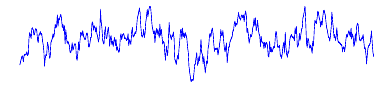
\includegraphics[width=\linewidth]{graphic/eeg_noise_clean}
    \caption{Czysty sygnał EEG}
    \end{subfigure}\hspace*{\fill}
    \begin{subfigure}{0.48\textwidth}
    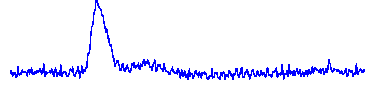
\includegraphics[width=\linewidth]{graphic/eeg_noise_blink}
    \caption{Mrugnięcie}
    \end{subfigure}
    
    \medskip
    \begin{subfigure}{0.48\textwidth}
    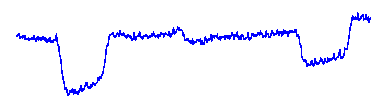
\includegraphics[width=\linewidth]{graphic/eeg_noise_eye}
    \caption{Ruch gałki ocznej}
    \end{subfigure}\hspace*{\fill}
    \begin{subfigure}{0.48\textwidth}
    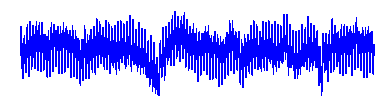
\includegraphics[width=\linewidth]{graphic/eeg_noise_line}
    \caption{Zakłócenia sieci energetycznej}
    \end{subfigure}
    
    \medskip
    \begin{subfigure}{0.48\textwidth}
    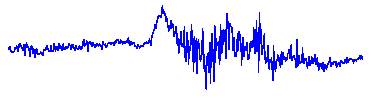
\includegraphics[width=\linewidth]{graphic/eeg_noise_muscle}
    \caption{Aktywność mięśni}
    \end{subfigure}\hspace*{\fill}
    \begin{subfigure}{0.48\textwidth}
    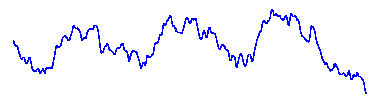
\includegraphics[width=\linewidth]{graphic/eeg_noise_pulse}
    \caption{Tętno}
    \end{subfigure}
    
    \caption{Rodzaje artefaktów występujących w sygnałach EEG\label{fig:eeg_noise}}
    \source{\cite{eeg_artifact}}
\end{figure}


\subsection{Ekstrakcja cech}
Celem ekstrakcji cech (\textit{ang.} feature extraction) jest przekształcenie \textit{surowych} danych EEG do postaci nadającej się do wykorzystania w procesie klasyfikacji sygnałów\cite{bci_robotics}.

Cecha jest właściwością opisującą sygnał EEG\cite{bci_foundations}. Cechą podstawową sygnału jest jego bezpośredni pomiar\cite{bci_principles}, na przykład różnica potencjałów pomiędzy dwoma elektrodami w chwili $t$. Podstawowe cechy są zazwyczaj przedstawiane w postaci cech złożonych, które stanowią ich liniowe oraz nieliniowe kombinacje, stosunki lub miary statystyczne. W celu jak najdokładniejszej detekcji intencji użytkownika wiele cech jest pozyskiwanych jednocześnie; są one zazwyczaj grupowane w tak zwane wektory cech\cite{bci_foundations}. 

Przykładem wykorzystania ekstrakcji cech może być rozpoznanie wyobrażenia ruchu ręką -- cechą używaną do detekcji jest moc pasma μ (8÷12 Hz) oraz β (16÷24 Hz)\cite{bci_foundations}.

W interfejsach mózg--komputer najczęściej wykorzystywane są cechy opisujące sygnał\cite{eeg_features}:
\begin{description}
    \item [Przestrzennie] --- służą do przybliżonego wyznaczania źródeł sygnału\cite{eeg_features}.
    \item [Spektralnie] --- opisują moc sygnału w zależności od częstotliwości\cite{bci_foundations}.
    \item [Czasowo] --- opisują zmianę sygnału w czasie.
\end{description}
Innymi cechami wykorzystywanymi w BCI są reprezentacje czasowo--czę\-sto\-tli\-wo\-ścio\-we sygnałów, transformacja Hilberta oraz parametry Hjortha\cite{bci_robotics}.

Problem ekstrakcji cech został poruszony szerzej w literaturze \cite{eeg_features,bci_foundations,bci_introduction,bci_robotics,bci_principles}.


\subsection{Klasyfikacja sygnałów}
Klasyfikatory służą do rozpoznawania wzorców w wektorach cech sygnałów EEG. Ich zadaniem jest przekształcenie aktywności mózgu w sygnały użyteczne dla komputera.

Wśród klasyfikatorów można wyróżnić między innymi:
\begin{description}
    \item [Klasyfikator liniowy] --- algorytm dyskryminacyjny posługujący się funkcjami liniowymi w celu rozróżnienia poszczególnych klas\cite{eeg_classification}. Wśród tego rodzaju klasyfikatorów w BCI najczęściej wykorzystywane są LDA\footnote{LDA (\textit{ang.} linear discriminant analysis) -- liniowa analiza dyskryminacyjna} oraz SVM\footnote{SVM (\textit{ang.} support vector machine) -- maszyna wektorów nośnych}\cite{bci_trends}.
    
    LDA jest liniowym klasyfikatorem binarnym, który przy pomocy hiperpłaszczyzny rozdziela dane reprezentujące różne klasy\cite{eeg_classification}. Metoda jest stosunkowo prosta i posiada małą złożoność obliczeniową, przez co jest często stosowana w BCI. Jej wadą jest osiąganie słabych rezultatów klasyfikacji w przypadku złożonych, nieliniowych wektorów cech sygnałów EEG\cite{bci_trends}. 

    SVM, podobnie jak LDA, używa hiperpłaszczyzny w celu rozdzielenia poszczególnych klas. W przypadku SVM poszukiwana hiperpłaszczyzna powinna rozdzielać z maksymalnym marginesem dane należące do odrębnych klas. Metoda posiada dobre właściwości generalizacji oraz jest niewrażliwa na przetrenowanie\cite{eeg_features}.

    \item [Sieci neuronowe] --- wśród sieci neuronowych wykorzystywanych w BCI najczęściej zastosowanie znajduje MLP\footnote{MLP (\textit{ang.} multilayer perceptron) -- wielowarstwowy perceptron}\cite{eeg_classification}.
    
    MLP składa się z kilku warstw neuronów: warstwy wejściowej, warstw ukrytych oraz warstwy wyjściowej. Wielowarstwowy perceptron jest wrażliwy na przetrenowanie, w szczególności w przypadku zaszumionych danych, takich jak sygnały EEG\cite{bci_trends}.

    Innymi rodzajami sieci neuronowych wykorzystywanymi w BCI są między innymi LVQ, Fuzzy ARTMAP, RBF oraz BLRNN, ALN oraz PeGNC\cite{eeg_classification}.
    
    \item [Naiwny klasyfikator bayesowski] --- jest klasyfikatorem probabilistycznym opartym na założeniu niezależności cech. Z tego powodu jest również zwany modelem cech niezależnych (\textit{ang.} independent feature model). Rozpatrując klasyfikację jako zadanie przyporządkowania klasy do konkretnego wejścia na podstawie wektorów cech $F_1$, $F_2$,\dots,$F_n$, decyzję otrzymujemy poprzez wybranie klasy z największym prawdopodobieństwem:
    $$P(C=i|F_1, \dots ,F_n)$$
    Na drodze przekształceń, korzystając z twierdzenia Bayesa, otrzymujemy prawdopodobieństwo w postaci:
    $$P(C=i|F_1, \dots ,F_n) = P(C=i)P(F_1|C=i)P(F_2|C=i) \dots P(F_n|C=i)$$
    Mając równanie w tej postaci, wynik klasyfikacji otrzymujemy poprzez obliczenie prawdopodobieństwa dla każdej z klas, a następnie wybranie tej o największym prawdopodobieństwie\cite{bci_introduction}.    

    \item [Algorytm najbliższego sąsiada] --- klasa wyjściowa jest przydzielana na podstawie najbliższego sąsiada, który jest wyłaniany na przykład przy pomocy odległości euklidesowej między wektorami, danej wzorem\cite{bci_introduction}: 
    $$d_{x,y} = \sqrt{\sum_{n=1}^{M}(x_n-y_n)^2}$$
    gdzie $d_{x,y}$ jest odległością między wektorami $x$ oraz $y$.

    Klasyfikacja algorytmem najbliższego sąsiada NN (\textit{ang.} nearest neighbor) jest podatna na szum\cite{bci_introduction}. Z tego powodu często jest zastępowana bardziej odporną odmianą w postaci algorytmu \textit{k} najbliższych sąsiadów k-NN (\textit{ang.} \textit{k} nearest neighbors), w którym klasa jest przyporządkowywana na podstawie klasyfikacji \textit{k} najbliższych sąsiadów.
\end{description}

W celu poprawy klasyfikacji można zastosować połączenie kilku różnych algorytmów. Ostateczne przyporządkowanie do konkretnej klasy następuje wtedy na drodze wzmacniania, głosowania lub nakładania.

Wzmacnianie (\textit{ang.} boosting) wykorzystuje klasyfikatory połączone w kaskadę. Każdy klasyfikator stara się wyeliminować błąd wprowadzony przez poprzednie. Ten sposób łączenia pozwala na stworzenie wydajnego klasyfikatora z połączenia kilku słabych. Charakteryzuje się odpornością na przetrenowanie\cite{bci_trends}.

Przy głosowaniu (\textit{ang.} voting) kilka klasyfikatorów samodzielnie dokonuje przydzielenia danych wejściowych do odpowiedniej klasy. Klasa wynikowa zostaje wyłoniona na drodze głosowania, to jest zostaje nią klasa, która została wyłoniona najwięcej razy podczas samodzielnych klasyfikacji.

Nakładanie (\textit{ang.} stacking) wykorzystuje dwa poziomy klasyfikatorów. Pierwszy, tak zwany poziom 0, klasyfikuje dane wejściowe do odpowiednich klas. Wyjścia klasyfikatorów poziomu 0 są połączone z wejściami klasyfikatora poziomu wyższego, zwanego poziomem 1, który podejmuje ostateczną decyzję dotyczącej przynależności do danej klasy\cite{eeg_classification}.

Połączone klasyfikatory uzyskują lepsze rezultaty. Ich połączenie obniża wariancję oraz błąd klasyfikacji\cite{eeg_classification}.


\section{Przegląd potencjalnych zastosowań}
\subsection{Interfejs komunikacyjny\label{subsec:p300}}
Najprostsze interfejsy komunikacyjne można zrealizować dając użytkownikowi do wyboru dwie opcje: \textit{tak} lub \textit{nie}. Podejście dwuwartościowe pozwala na stosowanie różnorodnych technik akwizycji wyboru, między innymi poprzez analizę mrugnięć, ruchu gałek ocznych, czy sygnałów pochodzących z BCI. Przy tak skonstruowanym interfejsie osoba z niego korzystająca jest w stanie odpowiadać na pytania rozmówcy.

Taki sposób komunikacji może być zmodyfikowany w celu umożliwienia osobie użytkującej interfejs nadawania toku rozmowy. Dzięki zastosowaniu tablicy ze znakami, jej rozmówca może przemieszczać  po kolei swój palec po literach alfabetu i notować te, dla których osoba korzystająca z interfejsu zakomunikowała odpowiedź \textit{tak}. Wadą takiego rozwiązania jest fakt, iż rozmówca musi asystować osobie niepełnosprawnej, co może wprowadzać uczestników rozmowy w zakłopotanie. Taki interfejs charakteryzuje się małą stopą błędu, jednak komunikacja przy jego użyciu jest długotrwała i wynosi około jedno słowo na minutę\cite{bci_trends}.

Innym podejściem jest stworzenie systemu opartego o wirtualny kursor, który pozwoliłby użytkownikowi na samodzielnie wybieranie liter lub całych wyrazów spośród dostępnych opcji. Taki system może zawierać elementy autokorekty, aby zminimalizować występujące błędy.

W literaturze można również spotkać się z systemami badającymi potencjały wywołane. Taką metodą jest \textit{P300}. W takim interfejsie użytkownik skupia swoją uwagę na literze, którą chce wybrać. Litery są samoczynnie podświetlane w losowej kolejności. 300 milisekund po podświetleniu litery, na której użytkownik systemu jest aktualnie skupiony, można zaobserwować zmianę amplitudy rejestrowanego sygnału EEG\cite{bci_introduction}. Przykładową realizację interfejsu opartego o analizę potencjału P300 pokazano na rysunku \vref{fig:p300_interface}.

\rysunek{p300}
{Struktura interfejsu opartego o potencjał P300\label{fig:p300_interface}}
{\cite{p300_interface}}


\subsection{Sterowanie wózkiem inwalidzkim}
Osoby sparaliżowane niekiedy są w stanie sterować wózkiem inwalidzkim, używając do tego celu wydmuchiwanego powietrza, mowy lub, w przypadku częściowego paraliżu, sprawnych części ciała. Integracja z interfejsami mózg--komputer stwarza nowe możliwości dla osób, które z powodu poważniejszych schorzeń nie są w stanie skorzystać z wyżej wymieniowych metod sterowania.

Kontrola wózka inwalidzkiego może odbywać się przy wykorzystaniu sterowania \textit{nisko-} lub \textit{wysokopoziomowego}.

Sterowanie niskopoziomowe można zrealizować przez translację sygnałów odebranych z urządzenia rejestrującego aktywność mózgu na komendy opisujące ruch wózka (\textit{ruch do przodu}, \textit{zawróć}, \textit{przyspiesz}), z zastrzeżeniem, że użytkownik wydaje je w sposób bezpośredni. Ten rodzaj sterowania wymaga zamontowania czujników na wózku, które uniemożliwią wykonanie niedozwolonych manewrów, na przykład uderzenia w inną osobę lub przedmiot. Do zalet rozwiązania można zaliczyć wysoki stopień kontroli osoby użytkującej wózek nad sposobem przemieszczania oraz stosunkowo małą ilość wymaganych komend mentalnych do podstawowego sterowania. Do wad należy konieczność wydawania poleceń ruchu w sposób ciągły, co może prowadzić do znużenia użytkownika, a w konsekwencji samoczynnego \textit{rozstrajania się} układu sterowania.

Sterowanie wysokopoziomowe polega na wydawaniu poleceń dotyczących celu ruchu (\textit{kuchnia}, \textit{łazienka}). Podejście to wiąże się z koniecznością stosowania wózków o wysokim stopniu autonomiczności. Zaletą tego rozwiązania jest odciążenie użytkownika od konieczności utrzymywania ciągłego skupienia na kierunku oraz prędkości ruchu, wyeliminowanie wpływu zakłóceń odbieranych w trakcie przemieszczania się oraz, po zapewnieniu skutecznych algorytmów i odpowiedniej ilości czujników, bezpieczniejsze poruszanie się w środowisku. Do wad zaliczyć należy większą ilość komend, które należy zdefiniować (co najmniej po jednej dla każdego pomieszczenia), mniejszą precyzję ruchu, spowodowaną odgórnym określeniem miejsca w pomieszczeniu, do którego użytkownik chce się przemieścić oraz konieczność zdefiniowania i zmapowania każdego środowiska, w którym będzie poruszał się wózek.

Mimo obiecujących wstępnych rezultatów, wykorzystanie interfejsów mózg--kom\-pu\-ter do zadania sterowania wózkami inwalidzkimi jest trudne do zrealizowania z powodu braku niezawodnych, przenośnych i łatwych w użyciu urządzeń rejestrujących. Inną przeszkodą jest brak wózków o wystarczającym stopniu autonomiczności, które byłyby zdalne do pracy w codziennym środowisku\cite{bci_introduction}.


\subsection{Rehabilitacja}
Można wyróżnić trzy główne sposoby wsparcia rehabilitacji medycznej przez interfejsy mózg--komputer\cite{bci_lab}:
\begin{description}
    \item [mózg--akcja] --- polega na nauczeniu pacjenta przy pomocy BCI wydawania odpowiednich poleceń, wymaganych do usprawnienia motoryki kończyn,
    \item [mózg--kończyna] --- polega na wykorzystaniu BCI do kontroli urządzenia wspierającego poruszanie się, a w konsekwencji odbudowania połączeń potrzebnych do poruszania się bez niego,
    \item [mózg--mózg] --- na podstawie informacji odebranych z systemu BCI następuje stymulacja mózgu w celu poprawy jego aktywności, aż do osiągnięcia zadowalających rezultatów.
\end{description}
Należy nadmienić, iż te sposoby nie są wzajemnie wykluczające -- ich połączenie pozwala na zwiększenie znaczenia BCI w tej dziedzinie nauki.

Interfejsy mózg--komputer, poprzez stopniową integrację z neurorehabilitacją, mogą pomóc między innymi osobom dotkniętym udarem mózgu, który często powoduje długotrwałą niepełnosprawność ruchową oraz zaburzenia funkcji poznawczych. Wiele badań wykazuje, iż technika nieinwazyjnej stymulacji mózgu jest skuteczna, nawet w przypadku przewlekłego uszkodzenia mózgu\cite{bci_lab}. Duża ilość osób rokrocznie dotykanych udarem stanowi badania w tym zakresie niezwykle istotnymi dla społeczeństwa.

Stosowanie BCI do wspomagania leczenia funkcji poznawczych wymaga skrupulatnej identyfikacji sygnałów mózgowych, które są możliwe do uzyskania. Może to być trudne, ponieważ nie wszystkie stany mózgu są tak dobrze scharakteryzowane, jak te związane z funkcjami motorycznymi\cite{bci_handbook}.


\subsection{Nadzór skupienia}
Wykorzystanie interfejsów mózg--komputer do nadzorowania skupienia użytkownika jest szczególnie istotne w asystowaniu pracowników wykonujących monotonne prace, takie jak prowadzenie samochodu czy monitorowanie systemu zabezpieczeń. Popełnienie błędu w przypadku takich profesji powoduje nie tylko ryzyko dla samego pracownika, ale również dla innych osób znajdujących się w jego otoczeniu. Wiele wypadków jest spowodowanych zmęczeniem, nieuwagą lub nawet zaśnięciem podczas wykonywania pracy. Choć znużenie lub senność może być wykryta przez analizowanie obszaru okolic oczu, taka detekcja może mieć miejsce za późno, aby było możliwe zapobiegnięcie wypadkowi. Integracja BCI z urządzeniami do nadzoru niesie możliwość wykrywania takich sytuacji, zanim doprowadzą do katastrofalnych w skutkach wydarzeń. 

W związku z postępującą automatyzacją pojazdów, kierowca jest odciążany od wykonywania żmudnych zadań, takich jak utrzymywanie stałej prędkości czy przełączanie między światłami mijania oraz drogowymi. Wraz z dalszym progresem coraz więcej czynności wykonywanych jest przez sam samochód, podczas kiedy rola osoby znajdującej się w fotelu kierowcy sprowadza się do nadzoru i reagowania w niebezpiecznych sytuacjach. Może to prowadzić, w szczególności na trasach o znacznej długości, do sytuacji nadmiernego zaufania do systemu sterowania, w której to kierowca przestanie zwracać uwagę na działania pojazdu. Interfejs mózg--komputer mógłby w tym momencie sygnalizować spadek skupienia kierowcy lub wymuszać bezpieczny postój pojazdu do momentu, w którym kierujący pojazdem będzie w stanie kontynuować podróż.

Badania przeprowadzone przez naukowców z \textit{Berlin BCI} wykazały, iż istnieje zależność pomiędzy spadkiem koncentracji, a wzrostem mocy w paśmie alpha\footnote{Pasmo alpha - pasmo fal elektromagnetycznych o częstotliwości 8÷12 Hz i amplitudzie w zakresie 20÷80 μV\cite[str. 17]{bci_handbook}.}\cite{bci_applications}. Badanie polegało na sklasyfikowaniu 2000 bagaży jako bezpiecznych lub niebezpiecznych na podstawie ich prześwietleń. Wykonano je w 10 turach po 200 bagaży. Zarejestrowaną zależność pomiędzy parametrem CII (\textit{ang.} concentration insufficiency index), a stopą błędu przedstawiono na rysunku \vref{fig:attention}. Na podstawie badania można wywnioskować, iż spadek koncentracji (wzrost parametru CII) prowadził do wzmożenia ilości popełnianych błędów. Uczestnicy rzeczonego badania na okres następujący bezpośrednio po przerwie wykazywali znacznie niższy stopień błędu. Tę zależność można wykorzystać do określenia momentów, w których pracownik powinien udać się na przerwę lub, w przypadku długotrwałej nikłej koncentracji, zakończyć swoją zmianę.

\rysunekbig[Zależność między stopniem skupienia, a stopą błędu]{attention}
{Zależność pomiędzy stopniem skupienia CII, a stopą błędu. Pionowe linie po zakończeniu dwustupróbkowych bloków oznaczają moment przerwy.\label{fig:attention}}
{\cite{bci_applications}}


\subsection{Gry komputerowe}
Wprowadzenie dedykowanych rozwiązań dla przemysłu gier komputerowych wydaje się być kolejnym krokiem po rozwoju aplikacji korzystających z technologii VR\footnote{VR (\textit{ang.} virtual reality) -- rzeczywistość wirtualna} oraz AR\footnote{AR (\textit{ang.} augmented reality) -- rzeczywistość rozszerzona}. To, co sprawia, że gracze są odpowiednim odbiorcą wczesnych systemów BCI jest fakt, iż często są oni zainteresowani nowymi technologiami, są skłonni do jej wdrażania w celu uzyskania przewagi nad przeciwnikami oraz przyzwyczajeni do konieczności treningu, który pozwala na progres w grach\cite{bci_games_survey}. W związku z dynamicznym rozwojem tej branży, opracowanie rozwiązań wykorzystujących BCI może być bardzo opłacalne w przyszłości.

Wykorzystanie BCI w grach komputerowych pozwala na integrację gry z wrażeniami użytkownika. Dostarczenie informacji na temat skupienia, zainteresowania, frustracji czy znudzenia umożliwia grze dostosowanie się do potrzeb gracza. W przypadku narastania frustracji gra może samoczynnie obniżyć poziom trudności, a w przypadku znudzenia -- podwyższyć. Wykorzystując inne odczucia gra może również uprościć interfejs użytkownika, czy też wyświetlić lub ukryć podpowiedzi dotyczące aktualnie wykonywanego zadania (\textit{ang.} quest). Dynamiczne dostosowywanie gry do aktualnego stanu gracza pozwala jej na zapewnienie użytkownikowi zwiększonego komfortu podczas rozgrywki.

Innym zastosowaniem interfejsów mózg--komputer jest wydawanie poleceń za pomocą komend mentalnych. Poleceniem może być na przykład wyobrażenie sobie ruchu postaci, co prowadziłoby do faktycznego przemieszczania się kontrolowanego bohatera, czy wybieranie odpowiedzi w dialogach występujących w grze. Wiąże się to z całkowitą zależnością gry od sygnałów otrzymywanych z urządzenia rejestrującego i wnosi konieczność znacznej modyfikacji istniejących silników gier.

Zintegrowanie BCI z grami komputerowymi wiąże się nie tylko ze znacznymi inwestycjami ze strony producentów gier, ale również samych graczy, którzy będą musieli zakupić urządzenia rejestrujące aktywność mózgu. Należy zwrócić uwagę na fakt, że rozgrywki często prowadzone są przez długi okres, a więc wymogiem stawianym przed systemami rejestrującymi jest ich wygoda. Nie mogą one ograniczać ruchów użytkownika ani jego pola widzenia. Wadą rozwiązania jest fakt, iż gracze często generują napięcia mięśniowe, co będzie prowadziło do powstawania artefaktów w przypadku urządzeń rejestrujących sygnały EEG. Rozwiązaniem tego problemu może być ulepszenie algorytmów filtracji sygnałów lub stosowanie systemów hybrydowych EEG/EMG, a więc rejestrujących oraz wykorzystujących aktywność zarówno mózgu, jak i mięśni\cite{bci_introduction}.


%%%%%%%%%%%%%%%%%%%%%%%%%%%%%%%%%%%%%%%%%%%%%%%%%%%%%%%%%%%%%%%%%%%%%%%%%%%%%%%%%%%%%%%%%%%%%%%%%%%%%%%%%%%%%%%%%%
%%%%%%%%%%%%%%%%%%%%%%%%%%%%%%%%%%%%%%%%%%%%%%%%%%%%%%%%%%%%%%%%%%%%%%%%%%%%%%%%%%%%%%%%%%%%%%%%%%%%%%%%%%%%%%%%%%
%%%%%%%%%%%%%%%%%%%%%%%%%%%%%%%%%%%%%%%%%%%%%%%%%%%%%%%%%%%%%%%%%%%%%%%%%%%%%%%%%%%%%%%%%%%%%%%%%%%%%%%%%%%%%%%%%%
\chapter{Charakterystyka wybranych urządzeń komercyjnych\label{chap:headsets}}
W rozdziale drugim zostały omówione wybrane urządzenia pozwalające na rejestrację aktywności mózgu. Zebrane urządzenia stanowią nieinwazyjne jednostki akwizycyjne, które są dostępne w sprzedaży detalicznej w cenie nieprzekraczającej 1000 \$. Przenalizowano sześć urządzeń czterech różnych producentów, w szczególności ich parametry, rodzaj oraz umiejscowienie czujników oraz dostępne narzędzia programistyczne. W przypadku każdego urządzenia wyszczególniono również jego cenę oraz, jeśli dotyczy, model licencjonowania.


\section{Emotiv Insight\label{section:insight}}
Insight (patrz rysunek \vref{fig:insight}) jest produktem wprowadzonym na rynek w roku 2015 przez firmę Emotiv przy wsparciu crowdfundingu na portalu \href{www.kickstarter.com}{kickstarter}. Jest produktem do użytku codziennego, głównie za sprawą minimalistycznego designu oraz braku konieczności stosowania żelów przewodzących, przeznaczonym do mniej precyzyjnych zastosowań.

Jest wyposażony w pięć czujników właściwych oraz dwa referencyjne. Lokalizacja czujników została przedstawiona na rysunku \vref{fig:insight_area}. Czas ubrania oraz ustawienia urządzenia oscyluje w granicach 1--2 minut. Parametry urządzenia zostały zestawione w tabeli \vref{tab:insight}.

Koszt produktu na dzień 21 kwietnia 2019 roku wynosi 299 \$.

\rysunek{insight}
{Hełm Emotiv Insight\label{fig:insight}}
{\cite{emotiv_insight}}

\rysunekbig{insight_area}
{Rozmieszczenie sensorów w hełmie Emotiv Insight\label{fig:insight_area}}
{\cite{emotiv_insight}}

\tabela{Parametry Emotiv Insight\label{tab:insight}}
{Opracowanie własne na podstawie \cite{emotiv_comparison}}
{
    \begin{tabular}{l|l}
        Ilość kanałów & 5 (+2 referencyjne)\\
        Umiejscowienie elektrod & AF3, AF4, T7, T8, Pz\\
        Czujniki referencyjne & DMS/DRL\\
        Rodzaj czujników & Półsuchy polimer\\
        Rozdzielczość & 14 bit na kanał\\
        Rozdzielczość LSB & 0,51 µV @ 14 bit\\
        Detekcja ruchu & 9-osiowy czujnik (3x żyroskop, 3x akcelerometr, 3x magnetometr)\\
        Łączność & Bezprzewodowa 2,4GHz/Bluetooth 4.0\\
        Zasilanie & Li-Pol 480 mAh, do 8 godzin pracy
    \end{tabular}
}

Firma Emotiv dostarcza do swoich rozwiązań API\footnote{API (\textit{ang.} application programming interface) -- Interfejs programistyczny aplikacji. Zawiera zestaw reguł i ich opisów, które definiują sposób komunikacji między programami komputerowymi.\label{foot:api}} o nazwie Cortex. Stanowi on podstawę do budowania aplikacji wykorzystujących pobrane z hełmów strumienie danych dzięki wykorzystaniu JSON oraz WebSocket\cite{emotiv_developer}. Cortex ułatwia tworzenie gier, aplikacji oraz rejestrowania danych do późniejszego ich wykorzystania do badań.

Cortex jest wrapperem SDK\footnote{SDK (\textit{ang.} software development kit) -- Zestaw narzędzi dla programistów niezbędny w tworzeniu aplikacji korzystających z danej biblioteki.\label{foot:sdk}} firmy EMOTIV. Zapewnia on, w zależności od rodzaju zakupionej licencji, dostęp do różnych strumieni danych z hełmów. Jest kompatybilny z systemami Mac OS oraz Windows. Umożliwia programowanie w językach Java, C\#, C++, Python, Ruby, JavaScript (Node.js) oraz PHP.

\pagebreak
Licencja Cortex jest dostępna w trzech planach omówionych poniżej.
\begin{description}
    \item [Darmowa] \hfill
    \begin{itemize}
        \item Mental Commands API,
        \item Performance Metrics API (do 0,1 Hz),
        \item Frequency Bands API,
        \item Facial Expressions API,
        \item Motion data API,
        \item nielimitowana ilość sesji na 3 urządzeniach.
    \end{itemize}
    \item [Niekomercyjna pro -- 55--99 \$/miesiąc] \hfill
    \begin{itemize}
        \item Wszystkie API z licencji darmowej,
        \item Raw EEG API,
        \item oprogramowanie EmotivPRO,
        \item nielimitowana ilość sesji na 3 urządzeniach.
    \end{itemize}
    \item [Komercyjna] \hfill
    \begin{itemize}
        \item Performance Metrics API o wysokiej rozdzielczości,
        \item konfigurowanie API pod swoje potrzeby,
        \item tworzenie komercyjnych rozwiązań.
    \end{itemize}
\end{description}

Oprogramowanie EmotivPRO\cite{emotiv_pro}, dostępne w licencjach niekomercyjnej pro oraz komercyjnej, stanowi wsparcie dla badań wykorzystujących EEG. Pozwala ono na akwizycję oraz prezentację strumieni danych w czasie zbliżonym do rzeczywistego, zapisywanie sesji w chmurze oraz szybką analizę wbudowanym algorytmem FFT\footnote{FFT (\textit{ang.} Fast Fourier Transform) -- Szybka transformacja Fouriera.}, bez konieczności eksportu danych.


\section{Emotiv EPOC+\label{section:epoc}}
EPOC+, pokazany na rysunku \vref{fig:epoc}, został wprowadzony na rynek w 2013 roku przez firmę Emotiv. Został zaprojektowany do badań wykorzystujących EEG oraz zaawansowanych zastosowań BCI\cite{emotiv_epoc}.

Jest wyposażony w 14 kanałów właściwych oraz 2 referencyjne (dokładna lokalizacja sensorów została przedstawiona na rysunku \vref{fig:epoc_area}). W odróżnieniu od Emotiv Insight, omówionego w rozdziale \vref{section:insight}, wymaga stosowania \textit{mokrych} elektrod, pokrytych nasączonym solą fizjologiczną filcem. Ze względu na większą ilość czujników niż w Emotiv Insight, czas ubrania oraz przygotowania urządzenia do pracy wynosi około 3--5 minut. Parametry hełmu zostały przedstawione w tabeli \vref{tab:epoc}.

Koszt produktu na dzień 21 kwietnia 2019 roku wynosi 799 \$.

\rysunek{epoc}
{Hełm Emotiv EPOC+\label{fig:epoc}}
{\cite{emotiv_epoc}}

\rysunekbig{epoc_area}
{Rozmieszczenie sensorów w hełmie Emotiv EPOC+\label{fig:epoc_area}}
{\cite{emotiv_epoc}}

\tabela{Parametry Emotiv EPOC+\label{tab:epoc}}
{Opracowanie własne na podstawie \cite{emotiv_comparison}}
{
    \begin{tabular}{l|l}
        Ilość kanałów & 14 (+2 referencyjne)\\
        Umiejscowienie elektrod & AF3, AF4, F3, F4, FC5, FC6, F7, F8, T7, T8, P7, P8, O1, O2\\
        Czujniki referencyjne & DMS/DRL\\
        Rodzaj czujników & Nasączane solą fizjologiczną\\
        Rozdzielczość & 14/16 bit na kanał\\
        Rozdzielczość LSB & 0,51 µV @ 14 bit/0,13 µV @ 16 bit\\
        Detekcja ruchu & 9-osiowy czujnik (3x żyroskop, 3x akcelerometr, 3x magnetometr)\\
        Łączność & Bezprzewodowa 2,4GHz/Bluetooth 4.0\\
        Zasilanie & Li-Pol 680 mAh, do 12 godzin pracy
    \end{tabular}
}

Od strony programistycznej urządzenie wykorzystuje to samo API oraz SDK co Emotiv Insight; zostały one omówione w rozdziale \vref{section:insight}.


\section{Muse/Muse 2}
Muse/Muse 2 są urządzeniami wspomagającymi medytację, które pozwalają na rejestrację w czasie rzeczywistym aktywności mózgu, tętna, oddechu oraz ruchu ciała\footnote{Rejestracja poszczególnych parametrów w zależności od wersji opaski.}\cite{muse2}. Przekształcają one zmierzoną aktywność mózgu w predefiniowane dźwięki, takie jak szum wody czy deszczu; w zależności od poziomu skupienia dźwięk będzie spokojny lub gwałtowny, co pozwala osobom uczącym się medytować na efektywniejszą naukę wyciszenia umysłu.

Oba urządzenia są z wyglądu bardzo do siebie podobne. Nowsze, Muse 2 (pokazane na rysunku \vref{fig:muse2}), w odniesieniu do poprzedniej wersji, zostało \textit{odchudzone}, przez co nabrało bardziej eleganckiego wyglądu oraz zyskało niższy profil z dodatkowymi czujnikami\cite{muse_comparison_article}. Dodano również miękkie w dotyku wykończenie.

\rysunek{muse2}
{Opaska Muse 2\label{fig:muse2}}
{\cite{muse2}}
  
Obie opaski są wyposażone w 7 czujników, w tym 3 referencyjne (patrz rysunek \vref{fig:muse_area}). Zestawienie parametrów oferowanych przez obie opaski znajduje się w tabeli \vref{tab:muse}.

\rysunekbig{muse_area}
{Rozmieszczenie sensorów w opasce Muse\label{fig:muse_area}}
{\cite{muse_specification}}

Koszt Muse wynosi 219 €; Muse 2 -- 269 €.

\tabela{Parametry Muse oraz Muse 2\label{tab:muse}}
{Opracowanie własne na podstawie \cite{muse_comparison} oraz \cite{muse_specification}}
{
    \begin{threeparttable}
        \begin{tabular}{l|l|l}
            Parametr & Muse & Muse 2 \\\hline\hline
            Ilość kanałów & 4 (+ 3 referencyjne) & 4 (+3 referencyjne)\\
            Umiejscowienie elektrod & TP9, AF7, AF8, TP10\tnote{a} & TP9, AF7, AF8, TP10\tnote{a} \\
            Czujniki referencyjne & CMS/DRL & CMS/DRL \\
            Rodzaj czujników & Suche srebrne/silikonowe & Suche srebrne/silikonowe \\
            Rozdzielczość & 12 bit na próbkę & 12 bit na próbkę \\
            Rejestrowane parametry & EEG & EEG, tętno, ruch ciała, oddech \\
            Kompatybilność & iOS, Android & iOS, Android \\
            Łączność & Bezprzewodowa Bluetooth 4.0 & Bezprzewodowa Bluetooth 5.0 \\
            Zasilanie & Li-Ion, do 5 godzin pracy & Li-Ion, do 5 godzin pracy \\
        \end{tabular}
        \begin{tablenotes}
            \item[a] \footnotesize Dokładna lokalizacja zależy od wielkości głowy użytkownika; zamieszczono lokalizację zgodną z \cite{muse_specification}. W literaturze można spotkać również T9, FP1, FP2, T10\cite{muse_article}.
        \end{tablenotes}
    \end{threeparttable}
}

Muse posiada oferty skierowane do następujących grup:
\begin{description}
    \item [\sout{Deweloperów}] --- na dzień 23 kwietnia 2019 roku Muse nie wspiera aktywnie swojego SDK\footnote{SDK -- Patrz przyp. \vref{foot:sdk}.}. Ostatnią dostępną wersją jest v6.0.3, wydana w marcu 2018 roku. Opaska Muse 2, z racji późniejszej daty premiery, \textbf{nie jest wspierana przez SDK}. Na stronie dla deweloperów\cite{muse_developer} znajduje się odnośnik do innych narzędzi, takich jak \href{https://choosemuse.com/muse-direct/}{Muse Direct} czy projektów open source, np. \href{https://github.com/alexandrebarachant/muse-lsl}{MuseLSL}, \href{https://github.com/NeuroTechX/eeg-notebooks}{EEG Notebooks}.

    \item [Profesjonalistów] --- w ramach subskrypcji Muse Connect profesjonaliści otrzymują program wspomagający rozwój ich biznesu poprzez uczenie ich klientów technik medytacji\cite{muse_professional}. W ten sposób otrzymują dostęp do różnych wskazówek m.in. webinariów\footnote{Webinarium -- Internetowe seminarium realizowane przy wykorzystaniu streamingu wideo.}, studiów przypadków oraz informacji, które pomogą wprowadzić Muse do ich biznesu. Muse Connect wspomaga prowadzenie podopiecznych: ustalanie dla nich celów do realizacji oraz śledzenie ich progresu (również w czasie rzeczywistym).

    Aplikacja oferuje dwa rodzaje subskrypcji:
    \begin{enumerate}
        \item miesięczną w cenie 39 \$/miesiąc,
        \item roczną w cenie 33 \$/miesiąc; w tej opcji dodatkowo otrzymujemy za darmo urządzenie Muse.
    \end{enumerate}

    \item [Naukowców] --- w ramach narzędzi dla naukowców Muse oferuje dostęp do MusePlayer oraz MuseLab. MusePlayer służy do rejestrowania, ponownego odtwarzania, przekierowywania oraz przetwarzania danych z opasek. Umożliwia konwersję z natywnego typu danych (.muse) na inne (.txt, .mat, .csv). MuseLab wykorzystuje się do wizualizacji danych.
\end{description}


\section{MindWave Mobile 2}
MindWave Mobile 2 zbudowane jest z opaski na głowę, klipsu na ucho oraz ramienia z zamocowanym czujnikiem (patrz rysunek \vref{fig:mindwave}). Elektrody referencyjne oraz uziemiające znajdują się na klipsie na uchu, a elektroda EEG na ramieniu dotykającym czoła w pozycji FP1. Umożliwia pomiar sygnałów EEG, sygnałów \textit{NeuroSky eSense}, na które składają się skupienie oraz medytacja, oraz mrugnięć. Do zasilania wykorzystywana jest pojedyncza bateria AAA, która starcza na 8 godzin pracy\cite{mindwave}.

Parametry urządzenia zostały zestawione w tabeli \vref{tab:mindwave}.

Koszt urządzenia na dzień 25 czerwca 2019 roku wynosi 100 \$.

\rysunekbig{mindwave}
{Hełm MindWave Mobile 2\label{fig:mindwave}}
{\cite{mindwave}}

\tabela{Parametry MindWave Mobile 2\label{tab:mindwave}}
{Opracowanie własne na podstawie \cite{mindwave}}
{
    \begin{tabular}{l|l}
        Ilość kanałów & 1\\
        Umiejscowienie elektrod & FP1\\
        Czujniki referencyjne & \textit{brak danych}\\
        Rodzaj czujników & \textit{brak danych}\\
        Rozdzielczość & 12 bit\\
        Częstotliwość próbkowania & 512 Hz\\
        Detekcja ruchu & Brak\\
        Łączność & Bezprzewodowa Bluetooth (BT/BLE)\\
        Zasilanie & 1,5 V (1 bateria AAA), do 8 godzin pracy
    \end{tabular}
}

NeuroSky dostarcza swoje API dla systemów iOS, Android, macOS oraz Windows. Darmowe narzędzia dla deweloperów składają się z trzech osobnych API\cite{mindwave_software}:

\begin{description}
    \item [ThinkGear Connector (TGC)] --- program działający w tle systemu operacyjnego; zarządza komunikacją z hełmem przy pomocy TCP/IP.
    \item [ThinkGear Communication Driver (TGCD)] --- biblioteka zawierająca funkcje pozwalające na połączenie oraz przetwarzanie danych z hełmu. Można ją wykorzystywać z językami C/C++, Java oraz C\#.
    \item [Protokół komunikacji MindSet] --- zawiera specyfikacje protokołu komunikacyjnego; pozwala na integrację hełmu z dowolną platformą/językiem programowania.
\end{description}

Dodatkowo można wykupić narzędzia dla naukowców w cenie 500 \$, na które składają się\cite{mindwave_research}:

\begin{description}
    \item [NeuroView] --- aplikacja do wyświetlania oraz zapisywania danych EEG w czasie rzeczywistym. Pozwala na rejestrację \textit{czystego} sygnału EEG, jego poszczególnych składowych oraz odczytów \textit{NeuroSky eSense} dla skupienia oraz medytacji. Umożliwia eksport do plików CSV.
    \item [NeuroSkyLab] --- aplikacja zapewniająca integrację ze środowiskiem MATLAB.
\end{description}


\section{OpenBCI Ultracortex \textit{Mark IV}\label{sec:markiv}}
Ultracortex, pokazany na rysunku \vref{fig:markiv}, jest open source'owym hełmem zaprojektowanym do pracy ze wszystkimi układami OpenBCI\cite{markiv_shop}. Pozwala na rejestrację sygnałów EEG, EMG oraz ECG. Wspiera do 16 kanałów rozmieszczonych na 35 różnych lokalizacjach według systemu 10-20\footnote{System 10-20 -- system opisu umiejscowienia elektrod; składa się z 21 elektrod. Podstawą tego standardu jest zdefiniowanie konturów między punktami orientacyjnymi czaszki (np. nasion, inion), a następnie podzielenie ich na proporcjonalne odległości 20\% całkowitej długości. Istnieją również systemy pokrewne, np. 10-10 oraz 10-5, które używają odpowiednio 10\% oraz 5\% całkowitej długości\cite[rozdz. 6]{bci_principles}.}.

W projekcie zastosowano \textit{suche} sensory EEG. Ich rozmieszczenie pokazano na rysunku \vref{fig:markiv_area}.

Czas założenia oraz uruchomienia hełmu wynosi poniżej 30 sekund.

Produkt można kupić w trzech wariantach:
\begin{enumerate}
    \item Do samodzielnego druku --- dostarczane są wszystkie części hełmu oprócz tych, które można wydrukować na drukarce 3D. Hełm należy zmontować samodzielnie na podstawie \href{https://docs.openbci.com/Headware/01-Ultracortex-Mark-IV#ultracortex-mark-iv-assembly-instructions}{dokumentacji}. Cena: 300--400 \$.
    \item Niezmontowany --- dostarczane są wszystkie części hełmu, również z tymi, które można wydrukować na drukarce 3D. Hełm należy zmontować samodzielnie na podstawie \href{https://docs.openbci.com/Headware/01-Ultracortex-Mark-IV#ultracortex-mark-iv-assembly-instructions}{dokumentacji}. Cena: 500--600 \$.
    \item Zmontowany --- dostarczany jest całkowicie zmontowany hełm. Cena: 700--850 \$.
\end{enumerate}

\rysunekbig{markiv}
{Hełm Ultracortex \textit{Mark IV}\label{fig:markiv}}
{\cite{markiv}}

\rysunekbig{markiv_area}
{Rozmieszczenie sensorów w hełmie Ultracortex Mark IV\label{fig:markiv_area}}
{\cite{markiv_shop}}

Dodatkowo należy zakupić wybraną płytkę OpenBCI. W dalszej części rozdziału zamieszczono opisy dostępnych układów. Parametry hełmu \textit{Mark IV} w połączeniu z kompatybilnymi płytkami zamieszczono w tabeli \vref{tab:markiv}.

\begin{description}
    \item [Ganglion Board] --- Ganglion (patrz rysunek \vref{fig:ganglion}) posiada 4 kanały, które mogą być użyte do mierzenia sygnałów EMG, EKG lub EEG\cite{ganglion_shop}. Częstotliwość próbkowania wynosi 200 Hz.

    \rysunek{ganglion}
    {OpenBCI Ganglion Board\label{fig:ganglion}}
    {\cite{ganglion_shop}}

    Komunikacja bezprzewodowa jest realizowana z wykorzystaniem \href{https://www.sparkfun.com/simblee}{Simblee BLE}, modułu Bluetooth 4.0 kompatybilnego z Arduino, który pozwala na łatwą integrację z IoT\footnote{IoT (\textit{ang.} Internet of Things) -- Internet rzeczy. Koncepcja zgodnie z którą urządzenia mogą komunikować się ze sobą, wykorzystując do tego celu internet.}. Moduł umieszczony na płytce Ganglion jest zaprogramowany i gotowy do pracy, jednak część jego wyprowadzeń pozostaje dostępna dla użytkownika do celów własnych.

    Koszt układu to 200 \$.

    \item[Cyton Board] --- Cyton, pokazany na rysunku \vref{fig:cyton}, jest kompatybilny z Arduino, posiada 8 kanałów oraz 32-bitowy procesor\cite{cyton_shop}. Podobnie jak Gangalion, może być wykorzystany do mierzenia aktywności mięśni, serca lub mózgu. Dane próbkowane są z częstotliwością 250 Hz.

    \rysunek{cyton}
    {OpenBCI Cyton Board\label{fig:cyton}}
    {\cite{cyton_shop}}

    Do komunikacji bezprzewodowej wykorzystywany jest moduł \href{https://eu.mouser.com/new/rfdigital/rf-digital-rfduino/}{RFduino}. Komunikacja z komputerem może być realizowana przy pomocy adaptera OpenBCI USB lub, jeżeli komputer posiada tę technologię, wbudowanego modułu BLE.

    Koszt płytki to 500 \$.

    \item[Cyton + Daisy Board] --- Ten układ zawiera opisaną wcześniej płytkę Cyton oraz Daisy, która jest \textit{wpinana} w płytkę Cyton. Układ pokazano na rysunku \vref{fig:cyton_daisy}.

    Daisy zapewnia dodatkowe 8 kanałów, które mogą być użyte do mierzenia EMG, EKG lub EEG\cite{cytondaisy_shop}. Częstotliwość próbkowania wynosi 250 Hz.

    \rysunek{cyton_daisy}
    {OpenBCI Cyton + Daisy Board\label{fig:cyton_daisy}}
    {\cite{cytondaisy_shop}}

    Koszt układu to 950 \$. Płytka Daisy nie może być zakupiona oddzielnie.
\end{description}

Oprogramowanie OpenBCI jest open source'owe i jest dostępne na \href{https://github.com/OpenBCI}{ich profilu na GitHubie}.

Głównym narzędziem do wizualizacji, nagrywania oraz komunikacji z płytkami jest OpenBCI GUI\cite{markiv_software_gui}. Narzędzie jest kompatybilne z systemami macOS, Windows oraz Linux. Pozwala na filtrowanie oraz przetwarzanie danych w czasie rzeczywistym; umożliwia również przekierowywanie danych wykorzystując protokoły UDP, OSC, LSL oraz port szeregowy.

Do komunikacji z układami stosowane są narzędzia OpenBCI Ganglion SDK oraz OpenBCI Cyton SDK, wykorzystujące protokół oparty na znakach ASCII\footnote{ASCII (\textit{ang.} American Standard Code for Information Interchange) -- siedmiobitowy system służący do kodowania znaków.}. OpenBCI dostarcza również bibliotekę Brainflow, która służy do analizy danych EMG, EKG oraz EEG\cite{markiv_software_brainflow}. Umożliwia ona programowanie w językach Python, Java, R, C++\footnote{Mimo iż biblioteka została napisana jest w C/C++, dodano nakładkę na język C++ w celu zapewnienia warstwy abstrakcji.}, Matlab oraz C\#.

Platforma OpenBCI umożliwia również współpracę z innymi programami do analizy sygnałów, m.in. \href{https://www.mathworks.com/products/matlab.html}{MATLAB}, \href{https://www.neuromore.com/}{Neuromore}, \href{http://openvibe.inria.fr/}{OpenVIBE}, \href{https://github.com/sccn/labstreaminglayer}{LabStreamingLayer} oraz \href{http://www.shifz.org/brainbay/}{BrainBay}.

\begin{landscape}
    \tabela{Parametry Ultracortex \textit{Mark IV} w połączeniu z kompatybilnymi układami\label{tab:markiv}}
    {Opracowanie własne na podstawie \cite{markiv_shop,ganglion_shop,cyton_shop,cytondaisy_shop}}
    {
        \begin{threeparttable}
            \begin{tabular}{l|l|l|l}
                Parametr & Ganglion & Cyton & Cyton + Daisy \\\hline\hline
                Ilość kanałów & 4 & 8 & 16\\
                Umiejscowienie elektrod & Konfigurowalne\tnote{a} & Konfigurowalne\tnote{a} & Konfigurowalne\tnote{a}\\
                Rodzaj czujników & Suche & Suche & Suche\\
                Rozdzielczość & 24 bit & 24 bit & 24 bit\\
                Częstotliwość próbkowania & 200 Hz & 250 Hz & 250 Hz\\
                Rejestrowane parametry & EMG, EKG, EEG\tnote{b} & EMG, EKG, EEG\tnote{b}  & EMG, EKG, EEG\tnote{b}\\
                Detekcja ruchu & 3 osiowy akcelerometr & 3 osiowy akcelerometr & 3 osiowy akcelerometr\\
                Kompatybilność & macOS, Windows, Linux & macOS, Windows, Linux & macOS, Windows, Linux\\
                Łączność & BLE 4.0 przez adapter & BLE & BLE\\
                Zasilanie & 6V (4 baterie AA) & 6V (4 baterie AA) & 6V (4 baterie AA)\\
            \end{tabular}
            \begin{tablenotes}
                \item[a] \footnotesize \textit{Mark IV} wspiera 35 lokalizacji według standardu 10-20. Punkty w których można umieścić elektrody pokazano na rysunku \vref{fig:markiv_area}.
                \item[b] \footnotesize Sensory nie są dołączane do płytek i należy je zakupić oddzielnie.
            \end{tablenotes}
        \end{threeparttable}
    }
\end{landscape}

%%%%%%%%%%%%%%%%%%%%%%%%%%%%%%%%%%%%%%%%%%%%%%%%%%%%%%%%%%%%%%%%%%%%%%%%%%%%%%%%%%%%%%%%%%%%%%%%%%%%%%%%%%%%%%%%%%
%%%%%%%%%%%%%%%%%%%%%%%%%%%%%%%%%%%%%%%%%%%%%%%%%%%%%%%%%%%%%%%%%%%%%%%%%%%%%%%%%%%%%%%%%%%%%%%%%%%%%%%%%%%%%%%%%%
%%%%%%%%%%%%%%%%%%%%%%%%%%%%%%%%%%%%%%%%%%%%%%%%%%%%%%%%%%%%%%%%%%%%%%%%%%%%%%%%%%%%%%%%%%%%%%%%%%%%%%%%%%%%%%%%%%
\chapter{Projekt wirtualnej klawiatury}
W rozdziale trzecim omówiono opracowaną aplikację. W pierwszej części rozdziału sformułowano założenia projektowe. Dalej omówiono zagadnienia związane z doborem narzędzi wymaganych do realizacji pracy, w tym urządzenia rejestrującego aktywność mózgu, języka programowania, środowiska programistycznego oraz systemu kontroli wersji. Kolejną częścią jest omówienie samej aplikacji, z wyszczególnieniem struktury jej kodu źródłowego, algorytmu działania, protokołu komunikacyjnego urządzenia rejestrującego, metodyki treningu detekcji komend mentalnych oraz procesu decyzyjnego aplikacji. Rozdział zawiera również omówienie interfejsu użytkownika.  

\section{Założenia projektowe}
Przed przystąpieniem do realizacji projektu wirtualnej klawiatury sformułowano założenia przedstawione poniżej.

\begin{enumerate}
    \item Aplikacja powinna umożliwiać wprowadzanie następujących znaków: liter A--Z, cyfr 0--9 oraz symboli przecinka i kropki. Powinna również umożliwiać wstawianie spacji, przejście do nowej linii oraz usunięcie ostatniego znaku.
    \item Wprowadzona wiadomość powinna być wyświetlana na interfejsie użytkownika. Wysłanie (zaakceptowanie) wiadomości powinno odczytać ją przy pomocy syntezatora mowy.
    \item Domyślnym językiem aplikacji powinien być język angielski.
    \item Nawigacja po klawiaturze oraz selekcja (wciśnięcie) poszczególnych klawiszy powinna odbywać się głównie z wykorzystaniem poleceń mentalnych. Opcjonalnie, jeżeli jest to konieczne, oprócz poleceń mentalnych mogą zostać wykorzystane do tego celu inne sygnały pozyskane z jednostki akwizycyjnej, na przykład EOG czy EMG.
    \item Aplikacja powinna umożliwiać sterowanie manualne (bez wykorzystania hełmu) w celu łatwego przetestowania algorytmów selekcji.
    \item Poszczególne parametry algorytmu obsługi klawiatury powinny być konfigurowalne dla użytkownika.
    \item Aplikacja powinna mieć zaimplementowany mechanizm zapisywania ostatnio sprecyzowanych parametrów algorytmu.
    \item Użytkownik aplikacji nie powinien musieć w sposób bezpośredni \textit{porozumiewać} się z API urządzenia; nie powinien w ogóle musieć znać jego protokołu komunikacyjnego.
    \item Aplikacja powinna mieć zaimplementowany mechanizm bezpośredniej wymiany wiadomości z urządzeniem, jednak jego użytkowanie powinno być całkowicie opcjonalne i niewymagane do sprawnej pracy z urządzeniem.
\end{enumerate}

\section{Wybór narzędzi}
\subsection{Urządzenia rejestrujące}
Wybierając urządzenie rejestrujące poszukiwano urządzenia, które (1) jest nieinwazyjne, (2) posiada rozwinięte SDK oraz bazę przykładowych aplikacji, (3) zapewnia sprzętowe wsparcie w zakresie detekcji komend mentalnych, (4) jest przystępne cenowo -- kosztuje poniżej 500 \$. Dodatkową zaletą urządzenia, aczkolwiek niewymaganą do realizacji niniejszej pracy, byłaby (6) możliwość rejestracji dodatkowych sygnałów, na przykład przy użyciu akcelerometru. Wyboru dokonywano spośród urządzeń omówionych w rozdziale \vref{chap:headsets}.

W przypadku OpenBCI Ultracortex \textit{Mark IV}, jednym z jego mankamentów jest wysoka cena -- nawet w przypadku zakupu najtańszego wariantu, a więc hełmu do samodzielnego druku oraz montażu wraz z układem Ganglion Board, cena wynosiła 500 \$. Po doliczeniu do tej kwoty wymaganych elektrod cena znacznie wzrasta. W przypadku oferowanego przez firmę OpenBCI \href{https://shop.openbci.com/collections/frontpage/products/d-i-y-neurotechnologists-starter-kit}{Starter Kitu}, który zawiera wszystkie wymagane peryferiale, cena wynosi blisko 950 \$. Samodzielność montażu w odczuciu autora pracy jest ryzykownym posunięciem w przypadku tak delikatnych oraz precyzyjnych urządzeń, tym bardziej że nie jest to standardowy model sprzedaży tej gamy urządzeń. Niewątpliwą zaletą urządzeń OpenBCI jest ich otwartoźródłowość -- oprogramowanie jest dostępne na serwisie \href{https://github.com/OpenBC}{GitHub}. Inną zaletą jest jego duża popularność oraz integracja z wieloma programami do analizy danych, jak na przykład MATLAB.

Urządzenia Muse 2 oraz MindWave Mobile 2 w odczuciu autora są narzędziami mało precyzyjnymi, nie nadającymi się do wykorzystania w celach badawczych. Ich zaletami jest łatwość nakładania, niska cena oraz \textit{smukłość}, która prawdopodobnie pozwala na długie sesję bez odczuwania dyskomfortu związanego z naciskiem urządzenia. Wadą Muse 2 jest brak SDK dla programistów. Wadą MindWave Mobile 2 jest liczba elektrod rejestrujących -- urządzenie jest wyposażone w wyłącznie jedną.

Emotiv Insight oraz EPOC+ są bardzo popularne wśród osób zajmujących się tematyką BCI. Za pomocą rozbudowanego API pozwalają na detekcję nie tylko aktywności mózgu w poszczególnych pasmach, ale również komend mentalnych oraz mimiki. Ze względu na wykorzystywany protokół komunikacyjny, są uniwersalne pod względem platformy programistycznej oraz języka programowania. Ich największym mankamentem jest brak darmowego dostępu do \textit{surowych} danych EEG -- żeby je uzyskać trzeba wykupić licencję. Urządzenie EPOC+ charakteryzuje się lepszymi parametrami niż Insight, jednak jest od niego droższe. Inną jego wadą jest rodzaj czujników; EPOC+ używa nasączanych solą fizjologiczną, podczas kiedy czujniki w Insight są wykonane z półsuchego polimeru.

Ostatecznie zakupiono urządzenie Emotiv Insight. Nabyto najnowszą wersję urządzenia; premiera modelu odbyła się w maju 2019 roku. Niniejsza praca jest jednym z pierwszych projektów powstających na jego nowej odsłonie. Głównym czynnikiem przemawiającym na jego korzyść był dostęp do zaawansowanego API, które dobrze wpasowuje się w założenia pracy. Urządzenie posiada również atrakcyjną cenę; w opinii autora spośród omówionych modeli Emotiv Insight zapewnia najlepszy stosunek ceny do oferowanych możliwości.


\subsection{Język programowania}
Wybierając język programowania poszukiwano języka, który (1) jest językiem wysokiego poziomu, (2) jest językiem obiektowym, (3) umożliwia łatwe tworzenie interfejsu użytkownika, (4) posiada kompleksową dokumentację, (5) charakteryzuje się potencjałem przyszłego rozwoju oraz (6) dużą popularnością. 

Języki wysokiego poziomu ułatwiają proces tworzenia oprogramowania, zwiększając czytelność kodu oraz poziom jego abstrakcji. Pozwalają na zdystansowanie się od warstwy sprzętowej komputera oraz większe skupienie się na aspektach związanych z logiką programu.

Języki obiektowe ułatwiają tworzenie dużych aplikacji. Programuje się w nich z użyciem obiektów, które stanowią instancje klas, które z kolei są definicją zmiennych, pól oraz metod dla obiektów danego typu. Wśród paradygmatów programowania obiektowego możemy wyróżnić abstrakcję, hermetyzację, polimorfizm oraz dziedziczenie.

Interfejs użytkownika umożliwia osobie użytkującej system na interakcję z oprogramowaniem. Wybrany język programowania powinien mieć zapewnioną łatwość tworzenia graficznych interfejsów; ich tworzenie powinno być możliwe natywnie, bez konieczności używania zewnętrznych bibliotek. 

Język powinien mieć kompleksową oraz dobrze sformułowaną dokumentację. Dokumentacja techniczna stanowi źródło częstych odniesień w procesie powstawania oprogramowania, a zatem powinna być łatwo dostępna i umożliwiać szybkie odnajdywanie w niej potrzebnych informacji.

Potencjał przyszłego rozwoju pozwoli autorowi na wykorzystanie umiejętności zdobytych w trakcie realizacji niniejszej pracy w przyszłym życiu zawodowym. Uwzględnienie tego kryterium przy wyborze danej technologii stanowi dobrą formę motywacji, która jest kluczowa do sprawnej realizacji pracy.

Używając języków o dużej popularności znacznie łatwiej jest posiłkować się serwisami dla programistów, takimi jak na przykład \href{www.stackoverflow.com}{Stack Overflow}. Dzięki swojej zaangażowanej społeczności, ułatwiają one proces rozwiązywania ewentualnych problemów, które mogą wystąpić w trakcie tworzenia oprogramowania.

Wśród wstępnie wyselekcjonowanych języków programowania znalazły się języki C++, C\#, Java oraz JavaScript.

JavaScript został wyeliminowany jako pierwszy, ze względu na fakt, iż interpretacja kodu w nim tworzonego jest zależna od przeglądarki internetowej. Wymusza to testowanie oprogramowania na różnych wersjach przeglądarek, co w efekcie wydłuża czas powstawania aplikacji. Inną wadą JavaScript jest brak dostępu do zaawansowanych technik debugowania, do których dostęp istnieje w przypadku języków kompilowanych.

C++, pomimo wielu dostępnych materiałów oraz zaawansowanego narzędzia do tworzenia interfejsów użytkownika w postaci \href{www.qt.io}{Qt}, został wykluczony ze względu na brak jego znajomości przez autora pracy.

Dokonując ostatecznego wyboru pomiędzy C\# oraz Javą, zdecydowano się zrealizować aplikację w języku C\#. Autor pracy posiada większe doświadczenie w pracy z tym językiem, przez co realizacja  w nim oprogramowania będzie w większym stopniu pozbawiona antywzorców oraz wykonana w zgodzie z ogólnie przyjętymi standardami. 

Wybranie języka C\# wiąże się również z wyborem technologii tworzenia interfejsu graficznego; wyboru dokonywano spośród Windows Forms (WinForms), Windows Presentation Foundation (WPF) oraz Universal Windows Platform (UWP). Zdecydowano się skorzystać z WPF ze względu na dodatkowe możliwości jakie oferuje pod kątem dostosowywania interfejsu użytkownika w odniesieniu do WinForms oraz brakiem ograniczeń, którymi charakteryzują się aplikacje uniwersalne\cite{winformswpfuwp}. 


\subsection{Środowisko programistyczne}
Najpopularniejszymi środowiskami programistycznymi do języka C\# są \href{https://visualstudio.microsoft.com/vs/}{Visual Studio}, \href{https://www.jetbrains.com/rider/}{Rider} oraz \href{https://code.visualstudio.com}{Visual Studio Code}.

Zarówno Visual Studio jak i Rider są bardzo zaawansowanymi środowiskami. Oba programy posiadają funkcjonalności usprawniające tworzenie kodu, jego debugowanie, integrację testów oraz zarządzanie projektem, co czyni je niezwykle potężnymi narzędziami do pracy z językiem C\#. W odczuciu autora główne różnice sprowadzają się do dwóch cech:
\begin{enumerate}
    \item Visual Studio posiada darmową wersję Community, podczas kiedy Rider, pomijając miesięczną wersję trial, wymaga zakupienia licencji,
    \item Rider zapewnia znacznie więcej funkcjonalności dotyczących inspekcji kodu, czyli wykrywania oraz zastępowania jego fragmentów w celu ich uproszczenia lub uniknięcia potencjalnych błędów\cite{rider}. 
\end{enumerate}

Visual Studio Code, pomimo iż z definicji jest edytorem kodu, a nie zintegrowanym środowiskiem programistycznym, posiada wiele funkcjonalności pełnoprawnego IDE. Posiada między innymi wsparcie dla debugowania kodu, wersjonowania oprogramowania, uzupełniania kodu oraz kolorowania składni. Jego możliwości mogą być powiększane przez obszerną bazę rozszerzeń. Do jego zalet zależy znaczna szybkość, przejrzysty interfejs oraz cross-platformowość. Wadami narzędzia są niskie możliwości w zakresie inspekcji kodu oraz debugowania. VS Code jest darmowe.

Ostatecznie zdecydowano się na zrealizowanie projektu, wykorzystując do tego celu Visual Studio. Rider został odrzucony ze względu na konieczność zakupienia licencji oraz jego krótki okres obecności na rynku, przez co opinie na jego temat mogą nie być obiektywne. Visual Studio Code nie zostało wybrane ze względu na swoje nikłe możliwości w zakresie refaktoryzacji kodu.

\subsection{System kontroli wersji}
Jako system kontroli wersji wybrano Git. Opracowana aplikacja jest hostowana w prywatnym, niedostępnym dla osób postronnych, repozytorium na serwisie \href{www.github.com}{GitHub}.

\section{Omówienie aplikacji}
\subsection{Struktura kodu źródłowego}
Rozwiązanie (\textit{ang.} Solution) zostało podzielone na dwa projekty: HeadsetController oraz VirtualKeyboard. Wydzielenie osobnych projektów odseparowało logikę związaną z obsługą samego hełmu oraz z wirtualną klawiaturą -- umożliwia to dołączanie projektu HeadsetController do innych aplikacji, nawet tych niewykonanych w języku C\#, bez konieczności ingerencji w jego kod. Struktura rozwiązania w postaci drzewa została przedstawiona na rysunku \vref{fig:solution_structure}.

\begin{figure}[!htb]
	\centering
    \begin{minipage}{\textwidth}
        \dirtree{%
        .1 Solution 'MSc'.
        .2 HeadsetController.
        .3 Headset/.
        .3 Services/.
        .4 API/.
        .5 Requests/.
        .5 Responses/.
        .5 Utils/.
        .2 VirtualKeyboard.
        .3 Converters/.
        .3 Models/.
        .3 Resources/.
        .3 Utilities/.
        .3 ValidationRules/.
        .3 ViewModels/.
        .3 Views/.
        .4 AttachedProperties/.
        .4 Controls/.
        }
    \end{minipage}\\
	\caption{Struktura rozwiązania przedstawiona w postaci drzewa\label{fig:solution_structure}}\source{Opracowanie własne}
\end{figure}


HeadsetController jest biblioteką służącą do komunikacji z urządzeniem. Jest projektem o typie wynikowym DLL\footnote{DLL (\textit{ang.} Dynamic-link library) -- biblioteka łączona dynamicznie; rodzaj biblioteki łączonej z programem dopiero w trakcie jego wykonywania.} (output type: class library). Nie stanowi samodzielnej aplikacji; jest przeznaczony do bycia dołączonym do innych projektów. W projekcie znajdują się dwa główne foldery: \path{Headset} oraz \path{Services}. 

Do folderu \path{Headset} należą klasy \path{Headset.cs} oraz \path{Insight.cs}. \path{Headset.cs} jest klasą abstrakcyjną realizującą niskopoziomową komunikację z urządzeniami Emotiv -- zajmuje się przetwarzaniem danych otrzymanych protokołem WebSocket, a następnie, na podstawie zawartości otrzymanej wiadomości, wywoływaniem odpowiednich eventów. \path{Insight.cs} stanowi programową reprezentację hełmu Emotiv Insight; umożliwia dostęp do jego parametrów, na przykład poziomu naładowania, jakości połączenia poszczególnych elektrod lub \textit{siły} komend mentalnych. Dziedziczy po klasie \path{Headset.cs}.

W folderze \path{Services} znajdują klasy \path{JsonParser.cs} oraz \path{WebSocket.cs}, które stanowią klasy opakowujące (\textit{ang.} wrappers) na operacje kolejno na formacie JSON oraz protokole WebSocket. Dzięki zastosowaniu takiego podejścia, wewnętrzna implementacja tych klas jest ukryta przed użytkownikami biblioteki. Dla programisty dostępne są wyłącznie wysokopoziomowe metody niezbędne do pracy z urządzeniem, co wpisuje się w zasadę hermetyzacji. W tym folderze znajduje się również folder \path{API}, który zawiera trzy podkatalogi: \path{Requests}, \path{Responses} oraz \path{Utils}. Pierwsze dwa z nich zawierają definicję zapytań oraz odpowiedzi, pogrupowanych w dalsze foldery zgodnie z nomenklaturą zawartą w \href{https://emotiv.gitbook.io/cortex-api/}{dokumentacji} protokołu komunikacyjnego urządzenia. Folder \path{Utils} zawiera klasę \path{Enums.cs}, w której umieszczone są typy wyliczeniowe wykorzystywane do komunikacji.

Projekt VirtualKeyboard jest aplikacją Windows (output type: Windows application) wykorzystującą strukturę interfejsu Windows Presentation Foundation (WPF). Zawiera 7 głównych folderów: \path{Converters}, \path{Models}, \path{Resources}, \path{Utilities}, \path{ValidationRules}, \path{ViewModels} oraz \path{Views}.

Katalog \path{Converters} zawiera implementacje interfejsów \lstinline[language={[Sharp]C}]{IValueConverter} oraz \linebreak \lstinline[language={[Sharp]C}]{IMultiValueConverter}. Są w nim zawarte konwertery umożliwiające stosowanie niestandardowej logiki do tworzenia powiązań między interfejsem użytkownika, a właściwościami (\textit{ang.} properties) w aplikacji. Przykładem zaimplementowanego konwertera może być \path{BooleanToVisibilityConverter.cs}, który zwraca wartość typu wyliczeniowego \lstinline[language={[Sharp]C}]{Visibility} na podstawie przekazanej zmiennej typu \lstinline[language={[Sharp]C}]{boolean}. I tak, dla parametru \lstinline[language={[Sharp]C}]{true} zwraca wartość \lstinline[language={[Sharp]C}]{Visibility.Visible}, a dla \lstinline[language={[Sharp]C}]{false} -- \lstinline[language={[Sharp]C}]{Visibility.Hidden}.

Folder \path{Models} zawiera klasy odpowiedzialne za logikę biznesową aplikacji. Umieszczona jest w nim klasa \path{Settings.cs}, przechowująca ustawienia dotyczące progów aktywacji dla poszczególnych komend mentalnych, czasu skupienia wymaganego do ich aktywacji oraz wartości określającej czy włączony został tryb offline aplikacji. Klasa jest deserializowana z pliku \path{settings.json} wraz ze startem aplikacji oraz serializowana do niego podczas jej zamknięcia. Dzięki zastosowaniu mechanizmu serializacji użytkownik nie traci ustawień poprzedniej sesji. W folderze \path{Models} znajduje się również definicja klasy \path{KeyboardNavigator.cs}, która odpowiada za proces decyzyjny dotyczący wyboru aktualnie zaznaczonego klawisza klawiatury oraz jego wciśnięcia.

Folder \path{Resources} zawiera graficzne zasoby wykorzystywane w aplikacji. Przechowywana jest tu między innymi ikona aplikacji -- \path{keyboard.ico}.

W katalogu \path{Utilities} znajduje się klasa \path{SettingsSerializer.cs}, która odpowiada za serializację oraz deserializację klasy \path{Settings.cs} oraz jej zapis/odczyt z pliku. Plik wynikowy \path{settings.json} zostaje umieszczony w folderze, w którym znajduje się aplikacja.

Folder \path{ValidationRules} zawiera klasę \path{NotEmptyValidationRule.cs}, która jest wykorzystywana do potwierdzenia poprawności wprowadzonych przez użytkownika ustawień połączenia z hełmem Emotiv Insight.

Katalog \path{ViewModels} zawiera tak zwane \textit{ViewModele}, czyli klasy implementujące interfejs \lstinline[language={[Sharp]C}]{INotifyPropertyChanged}, które stanowią centrum wykorzystywanego w aplikacji wzorca MVVM\footnote{MVVM (\textit{ang.} Model--View--ViewModel) -- wzorzec architektury oprogramowania zapewniający separację warstw UI oraz biznesowej; silnie zakorzeniony w aplikacjach WPF.}. Za pomocą mechanizmu komend oraz wiązania danych (\textit{ang.} data binding) są one połączone z widokami.

Ostatni katalog, \path{Views}, zawiera definicje widoków w postaci plików \lstinline[language={[Sharp]C}]{XAML}\footnote{XAML (\textit{ang.} Extensible Application Markup Language) -- oparty na XML język znaczników wykorzystywany do opisu interfejsu użytkownika w między innymi aplikacjach Windows Presentation Framework.}. Zawarte są w nim również foldery \path{AttachedProperties}, w których przechowywane są właściwości rozszerzające zdefiniowane kontrolki, oraz \path{Controls}, w którym znajduje się definicja stworzonej przez autora pracy kontrolki \path{KeyView}, która jest składową opracowanej klawiatury.  


\subsection{Algorytm działania}
Na rysunku \vref{fig:algorithm} przedstawiono schemat blokowy algorytmu aplikacji.

\begin{figure}
	\centering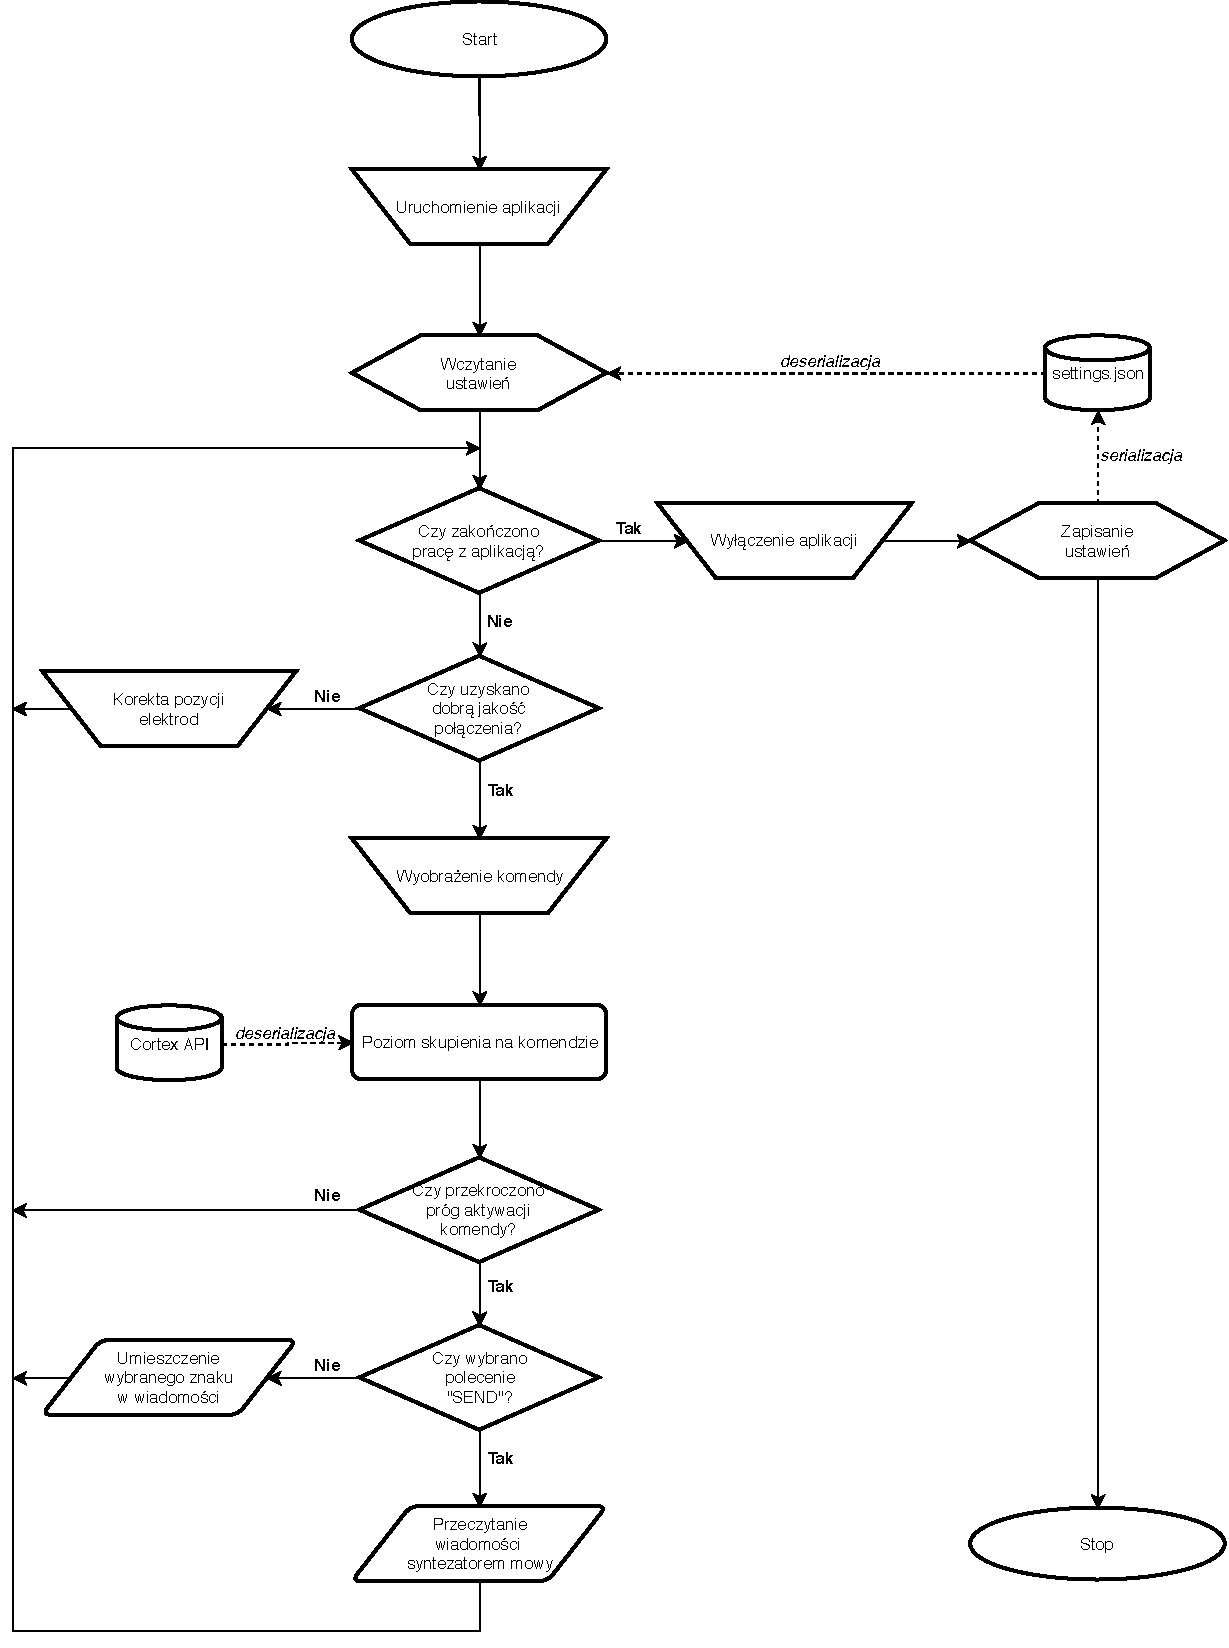
\includegraphics[height=\textheight,width=\textwidth,keepaspectratio]{graphic/flowchart.pdf}\\
	\caption{Schemat blokowy algorytmu aplikacji\label{fig:algorithm}}\source{Opracowanie własne}
\end{figure}

W momencie uruchomienia aplikacji następuje wczytanie ustawień zapisanych w pliku \path{settings.json}; plik zapisany jest w formacie JSON. W celu załadowania jego danych następuje deserializacja do obiektu klasy \path{Settings.cs}.

Po uruchomieniu aplikacji użytkownik powinien nałożyć hełm Emotiv Insight, dążąc przy tym do uzyskania jak najwyższej jakości sygnału. Jakość sygnału jest uśredniana do pojedynczej wartości procentowej oznaczonej na interfejsie użytkownika jako \textit{Contact Quality} (patrz rozdział \vref{subsec:virtualkeyboard}). Użytkownik może korygować położenie czujników na głowie, bazując na diagramie przedstawiającym głowę ze schematycznie oznaczonymi czujnikami, który został umieszczony w interfejsie użytkownika. Maksymalna możliwa do osiągnięcia jakość będzie różna w zależności od użytkownika; niezależnie od osiągniętych wartości praca z hełmem będzie możliwa, jednak im wyższa jakość połączenia, tym bardziej miarodajne będą sygnały odebrane z urządzenia.

W celu wykonania dowolnej komendy, a więc przesunięcia selekcji \textit{w górę}, \textit{w dół}, \textit{w prawo}, \textit{w lewo} lub \textit{wciśnięcia} klawisza, należy skupić się na danej akcji. Aplikacja, w momencie przekroczenia poziomu skupienia dla danej komendy zdefiniowanego w zakładce \textit{Settings}, wykona żądaną akcję. Jeżeli akcją będzie wciśnięcie klawisza z danym znakiem, zostanie on dodany do okna wiadomości znajdującego się w interfejsie użytkownika. Jeżeli akcją będzie wciśnięcie klawisza \textit{SEND}, tekst znajdujący się aktualnie w oknie wiadomości zostanie przeczytany przy użyciu syntezatora mowy, a następnie skasowany.

W momencie zamknięcia aplikacji wywoływana jest metoda zapisująca aktualnie zdefiniowane ustawienia. Odbywa się to poprzez serializację obiektu klasy \path{Settings.cs} do pliku \path{settings.json}.


\subsection{Trening detekcji komend mentalnych}
Poprzez swoje API Emotiv Insight umożliwia wykrywanie maksymalnie do 5 komend mentalnych, stanu neutralnego oraz wybranych czterech spośród następujących trzynastu wyobrażeń: pchnięcia, przyciągnięcia, uniesienia, opuszczenia, przesunięcia w lewo, przesunięcia w prawo, obrotu zgodnie ze wskazówkami zegara, obrotu przeciwnie do wskazówek zegara, obrotu w przód, obrotu w tył, obrotu w lewo, obrotu w prawo oraz zniknięcia. Dodatkowo wspomaga detekcję stanów emocjonalnych, to jest ekscytacji, długotrwałej ekscytacji, stresu, zaangażowania, odprężenia, zainteresowania oraz skupienia. Spośród mimiki umożliwia wykrywanie mrugnięcia, \textit{puszczenia oczka}, zmarszczenia brwi, uniesienia brwi, uśmiechu i zaciśnięcia zębów.

Wykorzystując aplikację EmotivBCI możliwe jest trenowanie detekcji poszczególnych komend mentalnych w czasie rzeczywistym. Trening jest interaktywny; użytkownik, obserwując wirtualny sześcian, \textit{wyobraża} sobie kolejne komendy, a system rejestruje aktywność mózgu związaną z danym wyobrażeniem. W miarę postępu oraz nasilania skupienia na danej akcji sześcian wykonuje wyobrażoną czynność, na przykład obraca się w prawo lub znika. Trening detekcji mimiki, podobnie jak komend mentalnych, jest również interaktywny -- użytkownik obserwuje postęp na wirtualnym awatarze. 

Istotną kwestią jest wybór odpowiednich poleceń mentalnych do obsługi wirtualnej klawiatury. Intuicyjność interakcji z systemem pozwoli użytkownikowi na szybsze przyswojenie zasady sterowania oraz zniweluje ilość błędów związanych z myleniem poleceń. Opracowany projekt wymaga pięciu komend: przesunięcia selekcji w górę, w dół, w prawo, w lewo oraz akceptację (\textit{wciśnięcie}) aktualnie oznaczonego klawisza. O ile w przypadku przesunięcia selekcji dobór komend mentalnych wydaje się oczywisty (są to polecenia \textit{uniesienie}, \textit{opuszczenie}, \textit{przesunięcie w lewo} i \textit{przesunięcie w prawo}), to komenda akceptacji wyboru wymaga głębszej analizy; czy powinno to być \textit{pchnięcie}, symulujące wciśnięcie klawisza klawiatury, a może \textit{przyciągnięcie}, czyli zwolnienie klawisza i przejście do wyboru kolejnej litery? Należy mieć również na uwadze, iż zwiększona ilość komend możliwych do wykrywania będzie prowadziła do powiększenia stopy błędu detekcji. Ponieważ w niniejszej aplikacji akceptacja selekcji jest kluczowym poleceniem, postanowiono wykorzystać do niego detekcję wyrazów twarzy. Zdecydowano, iż będzie za nią odpowiadać \textit{mrugnięcie}, które osiągało najkorzystniejszy stosunek poprawnych do omyłkowych klasyfikacji spośród dostępnych możliwości detekcji.

Zrzuty ekranu z procesu treningu komend pokazano na rysunku \vref{fig:training}. Na rysunkach \vref{fig:training_mental_all} oraz \vref{fig:training_facial_all} pokazano zestawienie wszystkich wytrenowanych modeli detekcji. Na rysunkach \vref{fig:training_mental_left} oraz \vref{fig:training_facial_blink} zaprezentowano zrzuty ekranu wykonane w trakcie rozpoznania przez aplikację \textit{EmotivBCI} wytrenowanych wzorców.

\begin{figure}
    \centering
    \begin{subfigure}[b]{0.475\textwidth}
        \centering
        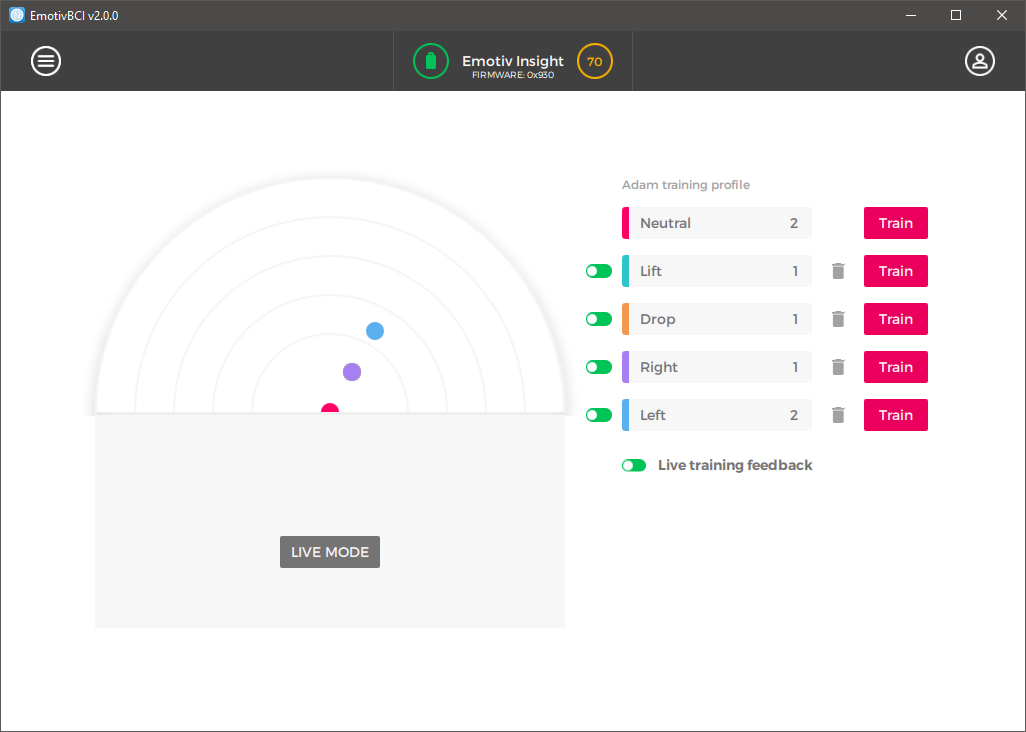
\includegraphics[width=\textwidth, keepaspectratio]{graphic/emotivbci_all}
        \caption{Zestawienie wszystkich wytrenowanych komend mentalnych\label{fig:training_mental_all}}
    \end{subfigure}
    \hfill
    \begin{subfigure}[b]{0.475\textwidth}  
        \centering 
        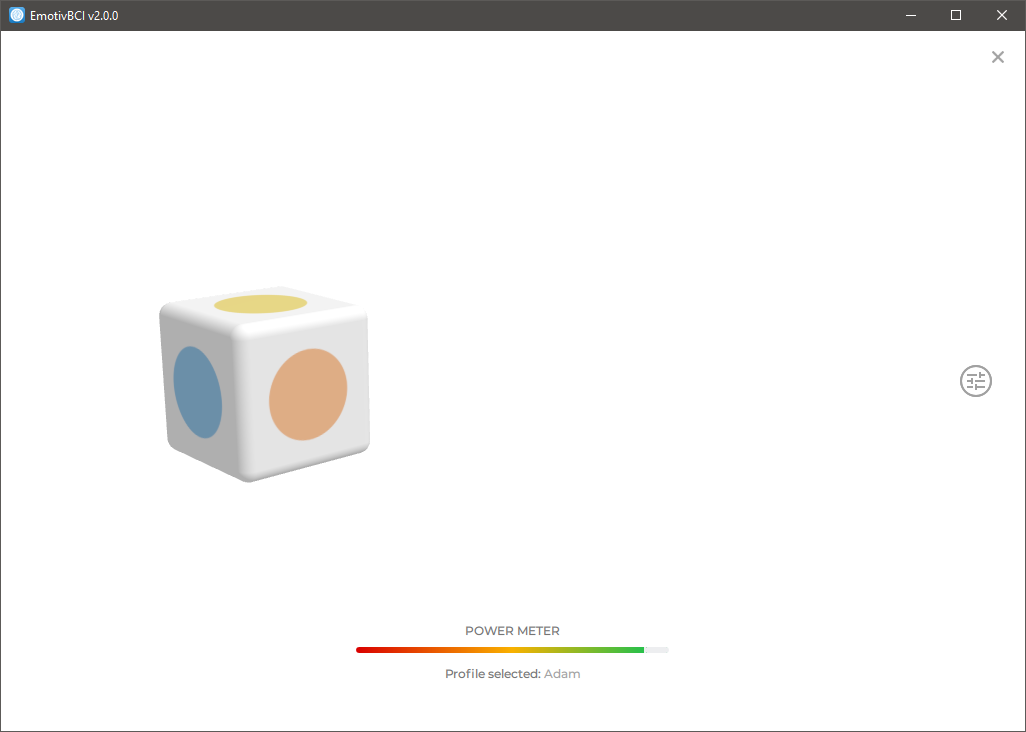
\includegraphics[width=\textwidth, keepaspectratio]{graphic/emotivbci_left}
        \caption{Obserwacja w trybie \textit{Live Mode} podczas wyobrażenia komendy \textit{w lewo}\label{fig:training_mental_left}}  
    \end{subfigure}
    \vskip\baselineskip
    \begin{subfigure}[b]{0.475\textwidth}   
        \centering 
        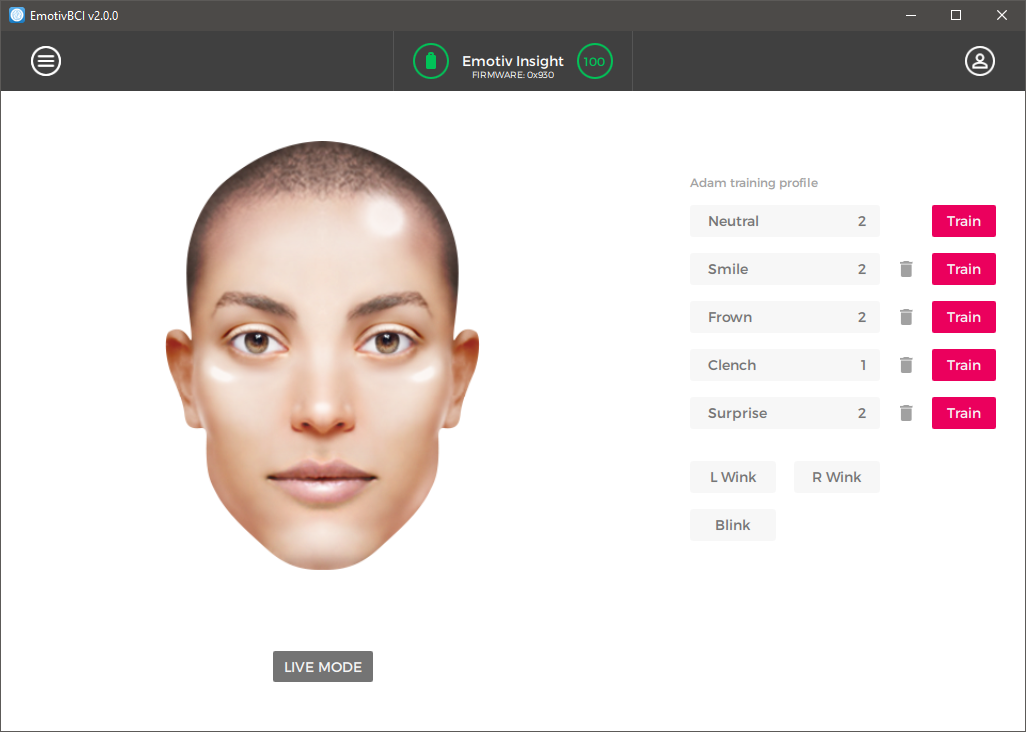
\includegraphics[width=\textwidth, keepaspectratio]{graphic/facial_all}
        \caption{Zestawienie wszystkich wytrenowanych detekcji mimiki\label{fig:training_facial_all}}  
    \end{subfigure}
    \quad
    \begin{subfigure}[b]{0.475\textwidth}   
        \centering 
        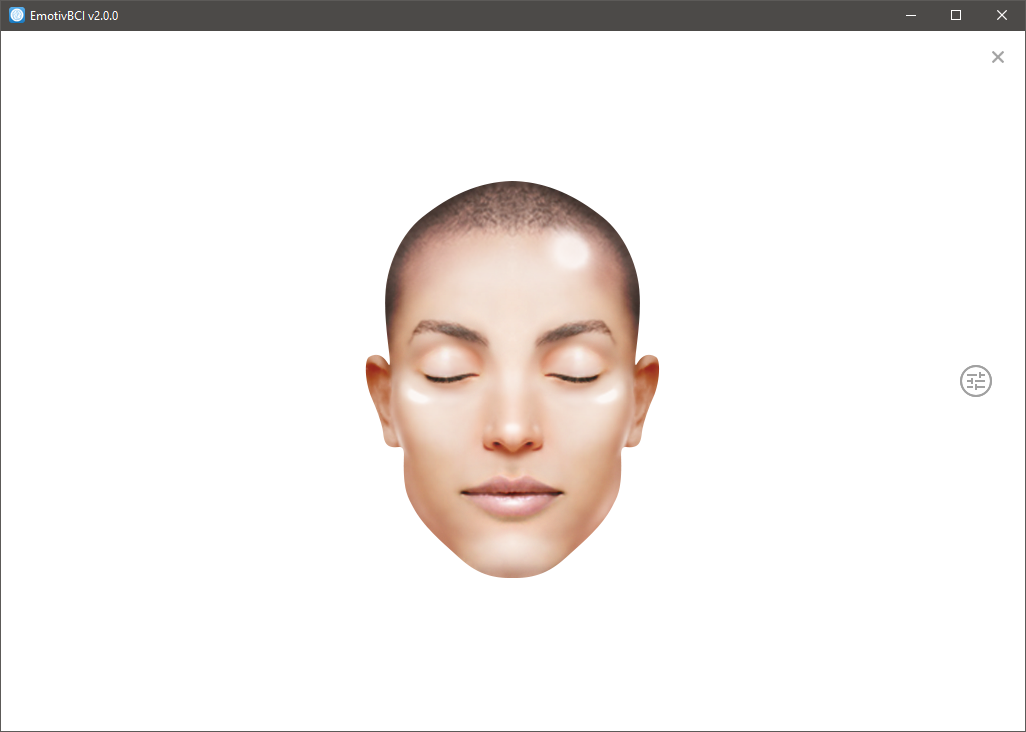
\includegraphics[width=\textwidth, keepaspectratio]{graphic/facial_blink}
        \caption{Obserwacja w trybie \textit{Live Mode} podczas wykonania akcji \textit{mrugnięcia}\label{fig:training_facial_blink}}   
    \end{subfigure}
    \caption{Proces treningu komend z wykorzystaniem aplikacji \textit{EmotivBCI}\label{fig:training}}
    \source{Opracowanie własne}
\end{figure}

\subsection{Komunikacja z urządzeniem}
Komunikacja z \href{https://emotiv.gitbook.io/cortex-api/}{Cortex API}, czyli wrapperem SDK Emotiv, odbywa się przy wykorzystaniu protokołu WebSocket oraz formatu danych JSON. Do nawiązania połączenia z hełmem wymagany jest Bluetooth w wersji 4.0 lub klucz sprzętowy USB (\textit{ang.} USB dongle).

W celu uzyskania identyfikatora aplikacji (\textit{ang.} application ID) koniecznego do wygenerowania identyfikatora klienta (\textit{ang.} client ID) oraz sekretu (\textit{ang.} client secret), zarejestrowano aplikację \textit{ict\_master} na stronie Emotiv; utworzono również konto EmotivID. Uzyskane w ten sposób dane umożliwiają autoryzację w Cortex API, pozwalając tym samym na otrzymywanie wyników wystosowanych zapytań.

Podczas uruchomienia aplikacji nawiązywane jest szyfrowane połączenie \textit{wss} (\textit{ang.} WebSocket Secure). Komunikacja odbywa się z wykorzystaniem protokołu \href{https://www.jsonrpc.org/specification}{JSON-RPC 2.0}, w którym każde zapytanie składa się z pól definiujących wersję JSON-RPC (\textit{jsonrpc}), nazwę wywoływanej metody (\textit{method}), jej parametrów (\textit{params}, o ile wymagane) oraz identyfikatora zapytania (\textit{id}). Otrzymany wynik zawiera specyfikację wersji JSON-RPC (\textit{jsonrpc}), wynik (\textit{result}) lub błąd (\textit{error}), oraz identyfikator zapytania (\textit{id}). Przykładowe zapytanie zostało pokazane na kodzie źródłowym \vref{code:sample_request}; przykładowa odpowiedź na nie znajduje się na kodzie źródłowym \vref{code:sample_response}.

\code{Przykładowe zapytanie Cortex API}{\cite{cortexdoc}}{\label{code:sample_request}}
\begin{lstlisting}[language=json]
{
    "id": 1,
    "jsonrpc": "2.0",
    "method": "authorize",
    "params": {
        "clientId": "xxx",
        "clientSecret": "yyy"
    }
}
\end{lstlisting}

\code{Przykładowy wynik zapytania Cortex API}{\cite{cortexdoc}}{\label{code:sample_response}}
\begin{lstlisting}[language=json]
{
    "id": 1,
    "jsonrpc": "2.0",
    "result": {
        "cortexToken":"zzz",
        "warning": {
            "code": 6,
            "message": "...",
            "licenseUrl": "https://..."
        }
    }
}
\end{lstlisting}

W celu minimalizacji liczby błędów komunikacji postanowiono zaimplementować kompletną bibliotekę zapytań oraz ich wyników. Opracowano w tym celu klasy \path{Request}, \path{Response} oraz klasy reprezentujące wszystkie możliwe zapytania, ich parametry oraz wyniki. 

Klasa \path{Request}, pokazana na kodzie źródłowym \vref{code:request}, stanowi klasę bazową dla wszy\-stkich zapytań Cortex API. Klasy zapytań, dziedzicząc po niej, uzyskują dostęp do zawartych w niej właściwości (\textit{ang.} properties). Dzięki temu zyskują mechanizm automatycznego przydzielania \textit{id} zapytania, którego niepowtarzalność jest kluczowa do poprawnej identyfikacji odebranych wyników; uzyskują również automatyczne przypisanie wersji protokołu JSON-RPC, która jest stała w obrębie Cortex API. Dodatkowo, dzięki zastosowaniu słowa kluczowego \lstinline[language=C]{abstract}, klasa bazowa wymusza redefinicję właściwości \lstinline[language={[Sharp]C}]{method}, która jest unikalna dla każdego rodzaju zapytania.

\vfill

\code{Kod klasy Request}{Opracowanie własne}{\label{code:request}}
\begin{lstlisting}[language={[Sharp]C}]
public abstract class Request : IRequest
{
    private static int _id;

    public int id { get; } = _id++;
    public string jsonrpc { get; } = "2.0";
    public abstract string method { get; }
}
\end{lstlisting}

\vfill

Przykładem klasy dziedziczącej po \path{Request} może być \path{AuthorizeRequest}. Jej kod został przedstawiony na kodzie źródłowym \vref{code:authorizeRequest}. Oprócz nadpisania w wierszu 3 właściwości \lstinline[language={[Sharp]C}]{method} wartością odpowiednią dla swojego zapytania, wprowadza ona właściwość \lstinline[language={C}]{@params}\footnote{W języku C\# \lstinline[language={C}]{params} jest słowem kluczowym i nie jest może być użyte jako identyfikator w programie, o ile nie zostanie poprzedzone prefiksem \lstinline[language={[Sharp]C}]{@}.} typu \lstinline[language={[Sharp]C}]{AuthorizeParameter}. 

\vfill

\code{Kod klasy AuthorizeRequest}{Opracowanie własne}{\label{code:authorizeRequest}}
\begin{lstlisting}[language={[Sharp]C}]
public class AuthorizeRequest : Request
{
    public override string method { get; } = "authorize";
    public AuthorizeParameter @params { get; }

    public AuthorizeRequest(AuthorizeParameter parameter)
    {
        @params = parameter;
    }
}
\end{lstlisting}

\vfill

Kod klasy \path{AuthorizeParameter} został pokazany na kodzie źródłowym \vref{code:authorizeParameter}. Poprzez swoją sygnaturę konstruktora, zawartą w wierszu 8, wymusza ona przekazanie parametrów, które są wymagane dla danego zapytania (\lstinline[language={[Sharp]C}]{clientId} oraz \lstinline[language={[Sharp]C}]{clientSecret}) na etapie tworzenia obiektu; parametry opcjonalne (\lstinline[language={[Sharp]C}]{license} oraz \lstinline[language={[Sharp]C}]{debit}) nie wymagają przekazania przez konstruktor i mogą pozostać nieprzydzielone.

\pagebreak

\code{Kod klasy AuthorizeParameter}{Opracowanie własne}{\label{code:authorizeParameter}}
\begin{lstlisting}[language={[Sharp]C}]
public class AuthorizeParameter
{
    public string clientId { get; }
    public string clientSecret { get; }
    public string license { get; set; }
    public int? debit { get; set; }

    public AuthorizeParameter(string clientId, string clientSecret)
    {
        this.clientId = clientId;
        this.clientSecret = clientSecret;
    }
}
\end{lstlisting}

\vfill

Kod klasy \lstinline[language={[Sharp]C}]{Response} został pokazany na kodzie źródłowym \vref{code:response}. Posiada on definicje wszystkich pól definiowanych przez standard JSON-RPC. W celu utworzenia jej instancji należy poprzez parametr generyczny \lstinline[language={[Sharp]C}]{T} sprecyzować jej typ, który musi implementować interfejs \lstinline[language={[Sharp]C}]{IResult}.

\vfill

\code{Kod klasy Response}{Opracowanie własne}{\label{code:response}}
\begin{lstlisting}[language={[Sharp]C}]
public class Response<T> where T : IResult
{
    public int id { get; }
    public string jsonrpc { get; }
    public T result { get; }

    [JsonConstructor]
    private Response(int id, string jsonrpc, T result)
    {
        this.id = id;
        this.jsonrpc = jsonrpc;
        this.result = result;
    }
}
\end{lstlisting}

\vfill

Przykładem implementacji interfejsu \lstinline[language={[Sharp]C}]{IResult} jest klasa \lstinline[language={[Sharp]C}]{AuthorizeResponse}, pokazana na kodzie źródłowym \vref{code:authorize_response}.

\pagebreak

Wysłanie zapytania odbywa się przy użyciu metody \lstinline[language={[Sharp]C}]{SendRequest} przedstawionej na kodzie źródłowym \vref{code:send_request}. Jako parametr przyjmuje ona zapytanie implementujące interfejs \lstinline[language={[Sharp]C}]{IRequest}, a więc wszystkie zapytania dziedziczące po klasie \lstinline[language={[Sharp]C}]{Request}. Wartością zwracaną jest \lstinline[language={[Sharp]C}]{Response<T>}, gdzie \lstinline[language={[Sharp]C}]{T} jest typem generycznym implementującym interfejs \lstinline[language={[Sharp]C}]{IResult}. W ciele tej metody odbywa się kojarzenie uzyskanych odpowiedzi z wysłanymi zapytaniami. W linii 13 następuje zasubskrybowanie wydarzenia (\textit{ang.} event) \lstinline[language={[Sharp]C}]{OnResponse}, dzięki czemu każdorazowe jego zgłoszenie spowoduje wywołanie lokalnej funkcji \lstinline[language={[Sharp]C}]{WaitResponseMatch}, w której, jeżeli \lstinline[language={[Sharp]C}]{id} zapytania oraz otrzymanej odpowiedzi są takie same, następuje odsubskrybowanie rzeczonej funkcji oraz przydzielenie otrzymanej odpowiedzi do wyniku zapytania. Ponieważ metoda \lstinline[language={[Sharp]C}]{SendRequest} jest asynchroniczna, nie blokuje ona interfejsu użytkownika w trakcie oczekiwania na odpowiedź.

\code{Kod klasy AuthorizeResponse}{Opracowanie własne}{\label{code:authorize_response}}
\begin{lstlisting}[language={[Sharp]C}]
public class AuthorizeResponse : IResult
{
    public string cortexToken { get; }
    public object warning { get; }

    [JsonConstructor]
    private AuthorizeResponse(string cortexToken, object warning)
    {
        this.cortexToken = cortexToken;
        this.warning = warning;
    }
}
\end{lstlisting}

\code{Kod metody SendRequest}{Opracowanie własne}{\label{code:send_request}}
\begin{lstlisting}[language={[Sharp]C}]
public async Task<Response<T>> SendRequest<T>(IRequest request) where T : IResult
{
    var tcs = new TaskCompletionSource<Response<T>>();

    void WaitResponseMatch(string response)
    {
        if (Parser.GetTokenAsString(response, "id") != request.id.ToString())
            return;

        OnResponse -= WaitResponseMatch; //unsubscribe after match
        tcs.SetResult(Parser.Deserialize<Response<T>>(response));
    }
    OnResponse += WaitResponseMatch;
    SendRequest(request);

    return await tcs.Task;
}
\end{lstlisting}

Na przykład, chcąc uzyskać Cortex Token, który jest niezbędny do autoryzacji większości zapytań Cortex API, należy wywołać metodę \lstinline[language={[Sharp]C}]{SendRequest}, przekazując do niej obiekt klasy \lstinline[language={[Sharp]C}]{AuthorizeRequest} z parametrem typu \lstinline[language={[Sharp]C}]{AuthorizeParameter}. Z uzyskanej odpowiedzi typu \lstinline[language={[Sharp]C}]{Response<AuthorizeResponse>} możliwe jest odczytanie \lstinline[language={[Sharp]C}]{cortexToken}. Operacje te, zawarte w metodzie \lstinline[language={[Sharp]C}]{Authorize}, pokazano na kodzie źródłowym \vref{code:request_response}. Wartością \lstinline[language={[Sharp]C}]{"xxx"} oznaczono \lstinline[language={[Sharp]C}]{clientId}, a \lstinline[language={[Sharp]C}]{"yyy"} \lstinline[language={[Sharp]C}]{clientSecret}.

\code{Kod metody Authorize}{Opracowanie własne}{\label{code:request_response}}
\begin{lstlisting}[language={[Sharp]C}]
public async Task Authorize()
{
    var authorizeResponse = SendRequest<AuthorizeResponse>(new AuthorizeRequest(new AuthorizeParameter("xxx", "yyy")));
    CortexToken = (await authorizeResponse).result?.cortexToken;
}
\end{lstlisting}

Wykorzystując wewnętrzny mechanizm serializacji zapytanie jest przekształcane do postaci pokazanej na kodzie źródłowym \vref{code:request_sent}, a następnie wysyłane przy użyciu protokołu WebSocket. Odpowiedź na to zapytanie została pokazana na kodzie źródłowym \vref{code:response_received}. Obie wiadomości są tożsame z przykładami zaczerpniętymi z dokumentacji, pokazanymi na kodach źródłowych \vref{code:sample_request} oraz \vref{code:sample_response}.

\code{Zserializowane zapytanie AuthorizeRequest}{Opracowanie własne}{\label{code:request_sent}}
\begin{lstlisting}[language=json]
{
    "method": "authorize",
    "params": {
        "clientId": "xxx",
        "clientSecret": "yyy"
    },
    "id": 1,
    "jsonrpc": "2.0"
}
\end{lstlisting}

\code{Odpowiedź otrzymana na zapytanie AuthorizeRequest}{Opracowanie własne}{\label{code:response_received}}
\begin{lstlisting}[language=json]
{
    "id": 1,
    "jsonrpc": "2.0",
    "result": {
        "cortexToken": "zzz"
    }
}
\end{lstlisting}


\subsection{Proces decyzyjny}
Proces decyzyjny, obejmujący zmianę selekcji aktualnie wybranego klawisza oraz jego \textit{wciśnięcie} (akceptację), odbywa się w oparciu o dane otrzymane od Cortex API. Po otwarciu sesji następuje zasubskrybowanie trzech strumieni danych: informacyjnego, komend mentalnych oraz mimiki. Subskrypcja powoduje przesyłanie w regularnych odstępach czasu obiektów w postaci formatu JSON. Zawartość wiadomości oraz jej częstotliwość zależą od rodzaju strumienia danych. Częstotliwość próbkowania dla strumienia informacyjnego, komend mentalnych oraz mimiki wynosi kolejno 128 Hz, 8 Hz oraz 32 Hz\cite{cortexdoc}.

O ile strumień informacyjny nie jest bezpośrednio wykorzystywany do podejmowania decyzji, tak informacje w nim zawarte są niezwykle istotne dla użytkownika urządzenia. Przesłane paczki zawierają dane na temat stanu hełmu: poziom naładowania jego baterii oraz jakość (siła) sygnału z poszczególnych czujników. Im lepsza łączność elektrod ze skórą głowy, tym wyniki pozostałych strumieni można uznać za bardziej miarodajne.

Dane strumieni komend mentalnych oraz mimiki mają zbliżony format, dlatego zostaną omówione na przykładzie wyłącznie jednej komendy -- wyobrażenia ruchu w prawo. Pozostałe komendy, czyli wyobrażenie ruchu w dół, w lewo, w górę oraz mrugnięcie, zostały zaimplementowane w analogiczny sposób.

Przy stworzeniu instancji klasy \lstinline[language={[Sharp]C}]{KeyboardNavigator} (patrz kod źródłowy \vref{code:keyboard_navigator}) następuje przekazanie do niej w konstruktorze obiektów \lstinline[language={[Sharp]C}]{Insight} oraz \lstinline[language={[Sharp]C}]{Settings}; referencje te zostają zapisane w klasie. Za sprawą interfejsu \lstinline[language={[Sharp]C}]{INotifyPropertyChanged}, implementowanego przez obie te klasy, następuje subskrypcja zmian wartości ich właściwości. W~konstruktorze następuje również ustawienie wartości czasomierza (\textit{ang.} timer) na wartość sprecyzowaną w zakładce \textit{Settings} oraz zasubskrybowanie wydarzenia informującego o upłynięciu odliczanego przez niego czasu.

\code{Kod konstruktora klasy KeyboardNavigator}{Opracowanie własne}{\label{code:keyboard_navigator}}
\begin{lstlisting}[language={[Sharp]C}]
public KeyboardNavigator(Insight insight, Settings settings)
{
    Insight = insight;
    Settings = settings;

    Insight.PropertyChanged += Insight_PropertyChanged;
    Settings.PropertyChanged += Settings_PropertyChanged;

    _rightTimer.Interval = TimeSpan.FromMilliseconds(Settings.FocusTime);
    _rightTimer.Tick += _rightTimer_Tick;
}
\end{lstlisting}

W momencie zgłoszenia wydarzenia \lstinline[language={[Sharp]C}]{PropertyChanged} przez obiekt \lstinline[language={[Sharp]C}]{Insight} następuje wywołanie metody \lstinline[language={[Sharp]C}]{Insight_PropertyChanged}, pokazanej na kodzie źródłowym \linebreak \vref{code:insight_propertychanged}. Metoda ta sprawdza jaka wartość została zmodyfikowana; jeżeli jest to siła skupienia na komendzie \textit{w prawo}, sprawdzane jest czy został przekroczony próg jej aktywacji, definiowany przez użytkownika w zakładce \textit{Settings}. Jeżeli tak -- następuje włączenie czasomierza \lstinline[language={[Sharp]C}]{_rightTimer}; jeżeli nie -- timer jest wyłączany.

\code{Kod metody Insight\_PropertyChanged}{Opracowanie własne}{\label{code:insight_propertychanged}}
\begin{lstlisting}[language={[Sharp]C}]
private void Insight_PropertyChanged(object sender, PropertyChangedEventArgs e)
{
    if (e.PropertyName == "RightLevel" && Insight.RightLevel >= Settings.RightThreshold)
        _rightTimer.Start();
    else if (e.PropertyName == "RightLevel")
        _rightTimer.Stop();
}
\end{lstlisting}

\vfill

Załączenie czasomierza, zgodnie z subskrypcją złożoną w kodzie źródłowym \vref{code:keyboard_navigator} w linii 10, powoduje wywołanie metody \lstinline[language={[Sharp]C}]{_rightTimer_Tick} co każde upłynięcie jego okresu, który, podobnie jak próg aktywacji poszczególnych komend, jest definiowany przez użytkownika w zakładce \textit{Settings}. Wywołana wtedy metoda, pokazana na kodzie źródłowym \vref{code:timer_tick}, zgłasza wydarzenie \lstinline[language={[Sharp]C}]{OnRightCommand}, które odpowiada za przesunięcie selekcji na klawiaturze o jeden klawisz w prawo.

\vfill

\code{Kod metody \_rightTimer\_Tick}{Opracowanie własne}{\label{code:timer_tick}}
\begin{lstlisting}[language={[Sharp]C}]
private void _rightTimer_Tick(object sender, EventArgs e) => OnRightCommand?.Invoke();
\end{lstlisting}

\vfill

W celu umożliwienia edycji ustawień w trakcie działania aplikacji (a nie wyłącznie na etapie jej uruchomienia) śledzone są również zmiany w klasie \lstinline[language={[Sharp]C}]{Settings}. Każdorazowa zmiana właściwości określającej częstość zgłaszania komend powoduje uaktualnienie wartości przypisanej do timera. Odpowiada za to metoda \lstinline[language={[Sharp]C}]{Settings_PropertyChanged}, pokazana na kodzie źródłowym \vref{code:settings_propertychanged}.

\vfill

\code{Kod metody Settings\_PropertyChanged}{Opracowanie własne}{\label{code:settings_propertychanged}}
\begin{lstlisting}[language={[Sharp]C}]
private void Settings_PropertyChanged(object sender, System.ComponentModel.PropertyChangedEventArgs e)
{
    if (e.PropertyName != "FocusTime")
        return;

    _rightTimer.Interval = TimeSpan.FromMilliseconds(Settings.FocusTime);
}
\end{lstlisting}

\vfill


\section{Omówienie interfejsu użytkownika}
\subsection{Zakładka \textit{Virtual Keyboard}\label{subsec:virtualkeyboard}}
Widok zakładki \textit{Virtual Keyboard} został pokazany na rysunku \vref{fig:virtual_keyboard}.

\rysunekwidth{virtual_keyboard}
{Widok zakładki \textit{Virtual Keyboard}\label{fig:virtual_keyboard}}
{Opracowanie własne}

\textit{Virtual Keyboard} jest domyślnym widokiem wyświetlanym po uruchomieniu aplikacji. Można w nim wydzielić cztery omówione poniżej segmenty.

\begin{description}
    \item [Moduł klawiatury] --- znajdująca się w lewym górnym rogu aplikacji klawiatura składa się z 42 klawiszy: liter A--Z, cyfr 0--9, znaków spacji, enter (przejście do nowej linii), przecinka, kropki, \textit{backspace} oraz znajdującego się w jej prawym dolnym rogu klawisza \textit{SEND}. Aktualnie wybrany klawisz jest oznaczany czerwoną ramką.
    
    Układ klawiatury jest rozwiązaniem autorskim, mającym na celu minimalizację liczby \textit{ruchów} potrzebnych do wprowadzenia wiadomości. Bazuje on na częstotliwości występowania liter w alfabecie angielskim, którą przyjął Samuel Morse opracowując swój alfabet\cite{morse}. Przyjętym przez autora priorytetem było (1) minimalizacja liczby ruchów oraz (2) minimalizacja liczby \textit{zakrętów} koniecznych do zaznaczenia danej litery, zakładając że poruszamy się ze środka klawiatury (litery \textit{E}).

    \item [Moduł okna wiadomości] --- znajduje się pod klawiaturą. Wyświetla tekst aktualnie wprowadzanej wiadomości. W momencie \textit{wyboru} znaku, jest on dodawany do wiadomości. Po wyborze klawisza \textit{SEND} następuje odczytanie tekstu wiadomości z użyciem syntezatora mowy, a następnie jego wyczyszczenie.
    
    \item [Moduł informacyjny] --- znajduje się w prawym górnym rogu aplikacji. Dostarcza w czasie rzeczywistym informacji na temat stanu Emotiv Insight: poziomu naładowania, jakości połączenia poszczególnych czujników oraz średniej jakości połączenia \textit{Contact Quality}. Dzięki schematycznemu przedstawieniu czujników na diagramie głowy, możliwe jest łatwe zlokalizowanie czujników o niskiej jakości połączenia, a następnie korekta ich powierzchni styku. W zależności od aktualnej jakości połączenia, kolor czujników będzie się zmieniał z czarnego przez czerwony, pomarańczowy aż do zielonego dla jakości połączenia kolejno bardzo złej, złej, dobrej oraz bardzo dobrej.
    
    \item [Moduł pada kierunkowego] --- pad kierunkowy (\textit{ang.} directional pad, d-pad) znajduje się w prawym dolnym rogu aplikacji. Składa się on z czterech strzałek kierunkowych oraz przycisku znajdującego się między nimi. 
    
    Poziom wypełnienia strzałki reprezentuje \textit{siłę} skupienia na odpowiadającej mu komendzie. Czerwoną linią został oznaczony próg aktywacji (\textit{ang.} threshold) komendy, po przekroczeniu którego następuje wykonanie powiązanej akcji. Użytkownik może edytować próg każdej z komend w zakładce \textit{Settings}. 

    Przycisk pomiędzy strzałkami odpowiada za \textit{wciśnięcie} (selekcję) aktualnie oznaczonego przycisku. Podobnie jak strzałki kierunkowe, threshold przycisku jest możliwy do edycji w zakładce \textit{Settings}. Skupienie się na komendzie selekcji jest sygnalizowane użytkownikowi przez wypełnianie okrągłego paska postępu znajdującego się wokół przycisku.
\end{description}


\subsection{Zakładka \textit{Messenger}}
Zakładka \textit{Messenger}, pokazana na rysunku \vref{fig:messenger}, umożliwia bezpośrednią wymianę wiadomości z Cortex API.

\rysunekwidth{messenger}
{Widok zakładki \textit{Messenger}\label{fig:messenger}}
{Opracowanie własne}

W górnej części okna znajduje się historia, zawierająca zarówno wysłane jak i odebrane wiadomości. Wiadomości dodawane są w kolejności chronologicznej zgodnie z następującym formatem: 
\begin{align*}
    &data \quad czas \quad typ:\\
    &tekst\\
\end{align*}
\begin{align*}
    \text{gdzie:}\\
    data &- \text{data wysłania/odebrania wiadomości w formacie DD-MM-RRRR}\\
    czas &- \text{czas wysłania/odebrania wiadomości w formacie HH-MM-SS.FFFF}\\
    typ  &- \text{typ wiadomości; sent lub received dla kolejno wysłanej lub odebranej}\\
    tekst &- \text{zawartość wiadomości}
\end{align*}

W oknie historii wyświetlane są zarówno wiadomości wysłane bezpośrednio przez użytkownika, jak i wszystkie wysłane podczas przez oprogramowanie podczas pracy aplikacji.

W dolnej części okna znajduje się pole do wpisywania wiadomości. Obok pola znajduje się przycisk służący do wysłania aktualnie wprowadzonego tekstu.


\subsection{Zakładka \textit{About}}
Widok zakładki \textit{About} został pokazany na rysunku \vref{fig:about}.

\rysunekwidth{about}
{Widok zakładki \textit{About}\label{fig:about}}
{Opracowanie własne}

Zawiera ona sekcje \textit{About}, zawierającą informacje na temat aplikacji: czym jest wirtualna klawiatura oraz czego używa do umożliwienia użytkownikowi interakcji z nią, \textit{Author}, przedstawiającą autora aplikacji oraz \textit{Get In Touch}, zawierającą odnośniki umożliwiające kontakt z autorem; są to odnośniki do \href{https://github.com/abaniuszewicz}{strony na GitHubie autora} oraz adresu e--mail.


\subsection{Zakładka \textit{Connection}}
Zakładka \textit{Connection} służy do definiowania ustawień połączenia z Cortex API. Jej widok przedstawiono na rysunku \vref{fig:connection}.

\rysunektwo
{connection_before}
{connection_after}
{Przed otwarciem sesji\label{fig:connection_before}}
{Po otwarciu sesji\label{fig:connection_after}}
{Widok zakładki \textit{Connection}\label{fig:connection}}
{Opracowanie własne}

Zawiera ona dwa pola tekstowe pozwalające na wprowadzenie \textit{Client ID} oraz \textit{Client Secret}, kluczy unikalnych dla opracowanej przez autora aplikacji. Dodatkowo zawiera dwie listy rozwijalne służące do wyboru hełmu oraz profilu użytkownika.

Pola w aplikacji posiadają weryfikację wprowadzonych danych; w przypadku wprowadzenia niepoprawnych wartości pole zostanie podkreślone na czerwono, a poniżej niego pojawi się komunikat błędu. Przykład działania tego mechanizmu pokazano na rysunku \vref{fig:connection_before} w polu \textit{Headset}.

Przycisk \textit{Refresh} pozwala na odpytanie Cortex API na temat znajdujących się w pobliży hełmów Emotiv oraz dostępnych profili. Po kliknięciu tego przycisku uzyskane dane są możliwe do wyboru z list rozwijalnych \textit{Headset} oraz \textit{Profile}.

Wykonanie operacji \textit{Create Session} jest możliwe wyłącznie w przypadku poprawnego sprecyzowania wszystkich dostępnych pól. Kliknięcie tego przycisku spowoduje otwarcie sesji z wybranym hełmem oraz zalogowanie na odpowiednim profilu. Po otwarciu sesji wszystkie kontrolki w tym widoku, za wyjątkiem przycisku służącego do zamknięcia sesji, stają się nieaktywne do momentu zakończenia sesji. Widok okna z otwartą sesją pokazano na rysunku \vref{fig:connection_after}.


\subsection{Zakładka \textit{Settings}}
Zakładka \textit{Settings} umożliwia użytkownikowi zmianę parametrów algorytmu aplikacji; jej widok pokazano na rysunku \vref{fig:settings}.

\rysunekbig{settings}
{Widok zakładki \textit{Settings}\label{fig:settings}}
{Opracowanie własne}

Przy użyciu zawartych w niej suwaków użytkownik może zmieniać próg aktywacji poszczególnych komend mentalnych. Wartość progu aktywacji wyrażona jest liczbą z zakresu $[0..1]$, przy czym $0$ oznacza bardzo niski próg, a $1$ bardzo wysoki.

Zakładka ta umożliwia dodatkowo zmianę parametru \textit{Command Focus Time}, definiującego czas przez który użytkownik musi skupić się na komendzie w poziomie przekraczającym jej threshold, aby powiązana z nią komenda została wykonana. Wartość czasu aktywacji wyrażona jest w milisekundach i może przyjmować wartości z zakresu $[1..2500]$.

Aktualna wartość definiowana przy pomocy suwaka jest widoczna po kliknięciu w niego; zostaje wtedy wyświetlony \textit{dymek} z jego aktualną wartością. Mechanizm ten został pokazany na rysunku \vref{fig:settings} przy polu \textit{Up Command Threshold}.

Na dole zakładki znajduje się przełącznik pozwalający na włączenie tak zwanego \textit{Offline Mode}. W tym trybie na oknie \textit{Virtual Keyboard} widoczne są suwaki, pozwalające na ręczną symulację aktualnego skupienia dla poszczególnych komend.

\chapter{Badania opracowanego systemu}
\section{Badanie wpływu zakłóceń}
\section{Badanie wpływu parametrów algorytmu}



\begin{zakonczenie}\label{chap:zakonczenie}
TODO
\end{zakonczenie}

% Bibliografia
\printbibliography[heading=bibintoc]

% Spis tabel (jeżeli jest potrzebny)
\listoftables

% Spis rysunków (jeżeli jest potrzebny)
\listoffigures

% Spis kodów źródłowych (jeżeli jest potrzebny)
\listoflistings

% TODO: Przenieść generowanie do pakietu glossaries i wyeliminować potrzebę manualnego wykonywania polecenia makeindex w terminalu. !! Dyskusyjne, indeksy należy definiować w preambule lub w osobnym pliku (tak samo jak acronyms), ale pozwala na większą swobodę w definiowaniu wpisów i nie wymaga wywoływania makeindex !!

% Skorowidz (opcjonalnie), po skompilowaniu dokumentu należy użyć opcji Narzędzia -> Indeks,
% aby wygenerować wpisy, po czym powtórnie skompilować dokument.
\printindex

\end{document}
